\documentclass[12pt,a4paper]{article}
\usepackage[utf8]{inputenc}
\usepackage[margin=1in]{geometry}
\usepackage{amsmath,amssymb,bm}
\usepackage{booktabs,array,makecell,tabularx}
\usepackage{graphicx}
\usepackage{float}
\usepackage{xcolor}
\usepackage{microtype}
\usepackage{cite}
\usepackage{enumitem}
\usepackage[section]{placeins}
\usepackage{hyperref}
\usepackage{xurl}
\hypersetup{colorlinks=true,linkcolor=blue!55!black,citecolor=blue!55!black,urlcolor=blue!55!black,pdftitle={Learning and Optimizing XGBoost with Planned Experiments},pdfauthor={Christos Chousein Sounios}}
% Auto-generated macros from genuine results
\newcommand{\envPlatform}{Windows-11-10.0.26300-SP0}
\newcommand{\numMeanFactorial}{0.6333}
\newcommand{\numMeanCenter}{0.4989}
\newcommand{\numDiffCurv}{0.1343}
\newcommand{\numSSCurv}{0.288786}
\newcommand{\numMSpeCenter}{2.74e-06}
\newcommand{\numDFpeCenter}{15}
\newcommand{\numFCurv}{105432.31}
\newcommand{\numICCAnova}{0.4069}
\newcommand{\numICCReml}{0.4069}
\newcommand{\numICCLatency}{0.0000}
\newcommand{\numFBlock}{20.21}
\newcommand{\numPBlock}{< 0.0001}
\newcommand{\numBzero}{0.4994}
\newcommand{\numTraceB}{0.133886}
\newcommand{\numSumEigs}{0.133886}
\newcommand{\numEigOne}{0.000057}
\newcommand{\numEigTwo}{0.000873}
\newcommand{\numEigThree}{0.022759}
\newcommand{\numEigFour}{0.110196}
\newcommand{\numFracMinEigLeZero}{68.2\%}
\newcommand{\numRsqRMSE}{0.9951}
\newcommand{\numAdjRsqRMSE}{0.9944}
\newcommand{\numAnovaPOneFxone}{357.40}
\newcommand{\numAnovaPOneEtxone}{0.8079}
\newcommand{\numAnovaPOneFxtwo}{23.57}
\newcommand{\numAnovaPOneFxoneXtwo}{26.32}
\newcommand{\numStationaryXone}{0.4171}
\newcommand{\numStationaryXtwo}{1.3524}
\newcommand{\numStationaryXthree}{15.6944}
\newcommand{\numStationaryXfour}{-6.8009}
\newcommand{\numStationaryYhat}{0.4161}
\newcommand{\numStationaryDistCoded}{17.16}
\newcommand{\numStationaryEta}{0.1113}
\newcommand{\numStationaryDepth}{9}
\newcommand{\numStationarySubsample}{1.0000}
\newcommand{\numStationaryLambda}{0.1000}
\newcommand{\numCubeOptDepth}{7}
\newcommand{\numCubeOptPredRMSE}{0.4483}
\newcommand{\numCubeOptEta}{0.1515}
\newcommand{\numCubeOptSubsample}{1.0000}
\newcommand{\numCubeOptLambda}{10.0000}
\newcommand{\numCubeOptXone}{0.5983}
\newcommand{\numCubeOptXtwo}{0.3333}
\newcommand{\numCubeOptXthree}{1.0000}
\newcommand{\numCubeOptXfour}{1.0000}
\newcommand{\vecBOne}{-0.1242}
\newcommand{\vecBTwo}{-0.0336}
\newcommand{\vecBThree}{-0.0047}
\newcommand{\vecBFour}{-0.0007}
\newcommand{\matBOneOne}{0.1065}
\newcommand{\matBOneTwo}{0.0169}
\newcommand{\matBOneThree}{-0.0024}
\newcommand{\matBOneFour}{-0.0048}
\newcommand{\matBTwoOne}{0.0169}
\newcommand{\matBTwoTwo}{0.0261}
\newcommand{\matBTwoThree}{-0.0019}
\newcommand{\matBTwoFour}{-0.0005}
\newcommand{\matBThreeOne}{-0.0024}
\newcommand{\matBThreeTwo}{-0.0019}
\newcommand{\matBThreeThree}{0.0006}
\newcommand{\matBThreeFour}{0.0005}
\newcommand{\matBFourOne}{-0.0048}
\newcommand{\matBFourTwo}{-0.0005}
\newcommand{\matBFourThree}{0.0005}
\newcommand{\matBFourFour}{0.0007}
\newcommand{\numBootLowEigOne}{-0.0039}
\newcommand{\numBootHighEigOne}{0.0022}
\newcommand{\numDfLofYone}{10}
\newcommand{\numDfPeYone}{111}
\newcommand{\numSSLofYone}{0.008850}
\newcommand{\numSSPeYone}{0.001579}
\newcommand{\numMSLofYone}{0.000885}
\newcommand{\numMSPeYone}{1.42e-05}
\newcommand{\numFLofYone}{62.21}
\newcommand{\numPLofYone}{7.78e-41}
\newcommand{\numSqrtMSLofYone}{0.0297}
\newcommand{\numSqrtMSPeYone}{0.0038}
\newcommand{\numBoxCoxYone}{-4.20}
\newcommand{\numDfPeCenter}{15}
\newcommand{\numSSPeCenterYone}{0.000041}
\newcommand{\numMSPeCenterYone}{2.74e-06}
\newcommand{\numSqrtMSPeCenterYone}{0.0017}
\newcommand{\numFLofCenterYone}{323.10}
\newcommand{\numPLofCenterYone}{1.22e-15}
\newcommand{\numDfInteract}{96}
\newcommand{\numSSInteractYone}{0.001538}
\newcommand{\numMSInteractYone}{1.60e-05}
\newcommand{\numSqrtMSInteractYone}{0.0040}
\newcommand{\numFInteractCenterYone}{5.85}
\newcommand{\numPInteractCenterYone}{0.0002}
\newcommand{\numSSPeCenterYtwo}{4148.89}
\newcommand{\numMSPeCenterYtwo}{276.59}
\newcommand{\numSqrtMSPeCenterYtwo}{16.63}
\newcommand{\numFLofCenterYtwo}{1.20}
\newcommand{\numPLofCenterYtwo}{0.3625}
\newcommand{\numSSInteractYtwo}{27844.93}
\newcommand{\numMSInteractYtwo}{290.05}
\newcommand{\numSqrtMSInteractYtwo}{17.03}
\newcommand{\numFInteractCenterYtwo}{1.05}
\newcommand{\numPInteractCenterYtwo}{0.4906}
\newcommand{\numLofRestrictedReductionPct}{96.3\%}
\newcommand{\numFLofRestricted}{10.11}
\newcommand{\numPLofRestricted}{1.30e-04}
\newcommand{\numSqrtMSLofRestricted}{0.0127}
\newcommand{\numSSLofRestricted}{0.000324}
\newcommand{\numDfLofYtwo}{10}
\newcommand{\numDfPeYtwo}{111}
\newcommand{\numFLofYtwo}{1.15}
\newcommand{\numPLofYtwo}{0.3305}
\newcommand{\numSqrtMSLofYtwo}{18.23}
\newcommand{\numSqrtMSPeYtwo}{16.98}
\newcommand{\numShapiroW}{0.9971}
\newcommand{\numShapiroP}{0.9947}
\newcommand{\numLeveneW}{0.1754}
\newcommand{\numLeveneP}{0.9507}
\newcommand{\numBrownForsytheW}{0.6872}
\newcommand{\numBrownForsytheP}{0.8552}
\newcommand{\numBreuschPaganLM}{70.10}
\newcommand{\numBreuschPaganP}{< 0.0001}
\newcommand{\numMaxCooksD}{0.097}
\newcommand{\numThreshFourN}{0.029}
\newcommand{\numOutlierCount}{9}
\newcommand{\numDurbinWatson}{1.9918}
\newcommand{\numLjungBoxStat}{4.01}
\newcommand{\numLjungBoxP}{0.5486}
\newcommand{\numRunsTestP}{0.8576}
\newcommand{\numOptDepth}{4}
\newcommand{\numOptEta}{0.2324}
\newcommand{\numOptSubsample}{1.0000}
\newcommand{\numOptLambda}{0.8295}
\newcommand{\numOptD}{0.6782}
\newcommand{\numOptdOne}{0.8783}
\newcommand{\numOptdTwo}{0.5236}
\newcommand{\numPredRMSE}{0.4804}
\newcommand{\numPredLatency}{138.11}
\newcommand{\numOptXone}{0.8500}
\newcommand{\numOptXtwo}{-0.6667}
\newcommand{\numOptXthree}{1.0000}
\newcommand{\numOptXfour}{-0.0812}
\newcommand{\numConfOptEta}{0.2324}
\newcommand{\numConfOptDepth}{4}
\newcommand{\numConfOptSubsample}{1.0000}
\newcommand{\numConfOptLambda}{0.8295}
\newcommand{\numConfLeverageH}{0.1043}
\newcommand{\numConfPredValRMSE}{0.4804}
\newcommand{\numConfPiLowValRMSE}{0.4677}
\newcommand{\numConfPiHighValRMSE}{0.4932}
\newcommand{\numConfNuEffMo}{14.0}
\newcommand{\numConfEmpValRMSE}{0.4853}
\newcommand{\numConfEmpValRMSEStd}{0.0115}
\newcommand{\numConfEmpTestRMSE}{0.4888}
\newcommand{\numConfEmpTestRMSEStd}{0.0032}
\newcommand{\numConfPredLat}{138.11}
\newcommand{\numConfPiLowLat}{122.82}
\newcommand{\numConfPiHighLat}{153.40}
\newcommand{\numConfEmpLat}{142.33}
\newcommand{\numConfEmpLatStd}{7.79}
\newcommand{\numConfPassValRMSE}{Pass (Inside 95\% PI)}
\newcommand{\numConfPassLat}{Pass (Inside 95\% PI)}
\newcommand{\numConfSoPredValRMSE}{0.4483}
\newcommand{\numConfSoPiLowValRMSE}{0.4354}
\newcommand{\numConfSoPiHighValRMSE}{0.4612}
\newcommand{\numConfSoNuEffSo}{15.1}
\newcommand{\numConfSoEmpValRMSE}{0.4700}
\newcommand{\numConfSoEmpValRMSEStd}{0.0093}
\newcommand{\numConfSoEmpTestRMSE}{0.4691}
\newcommand{\numConfSoEmpTestRMSEStd}{0.0034}
\newcommand{\numConfSoEmpLat}{171.1}
\newcommand{\numConfSoEmpLatStd}{10.9}
\newcommand{\numConfSoBias}{+0.0217}
\newcommand{\numDoeTestRMSE}{0.4884}
\newcommand{\numDoeValRMSE}{0.4821}
\newcommand{\numDoePredictLat}{119.8}
\newcommand{\numDoeInplaceLat}{87.1}
\newcommand{\numDoeSoTestRMSE}{0.4690}
\newcommand{\numDoeSoValRMSE}{0.4687}
\newcommand{\numDoeSoPredictLat}{147.8}
\newcommand{\numDoeSoInplaceLat}{116.9}
\newcommand{\numTpeTestRMSE}{0.4726}
\newcommand{\numTpeValRMSE}{0.4735}
\newcommand{\numTpePredictLat}{193.2}
\newcommand{\numTpeInplaceLat}{160.9}
\newcommand{\numRsTestRMSE}{0.4707}
\newcommand{\numRsValRMSE}{0.4696}
\newcommand{\numRsPredictLat}{198.1}
\newcommand{\numRsInplaceLat}{164.2}
\newcommand{\numMoTpeTestRMSE}{0.4870}
\newcommand{\numMoTpeValRMSE}{0.4812}
\newcommand{\numMoTpePredictLat}{118.8}
\newcommand{\numMoTpeInplaceLat}{87.6}
\newcommand{\numConstrainedTpeTestRMSE}{0.4823}
\newcommand{\numConstrainedTpeValRMSE}{0.4783}
\newcommand{\numConstrainedTpePredictLat}{125.4}
\newcommand{\numTestGapPct}{3.3\%}
\newcommand{\numLatSlowPct}{61.3\%}
\newcommand{\numDoeLatLowerPct}{38.0\%}
\newcommand{\numHvDoe}{16.50}
\newcommand{\numHvDoeSingle}{14.53}
\newcommand{\numHvMoTpe}{14.82}
\newcommand{\numHvRs}{6.71}
\newcommand{\numHvDoeGainPct}{11.4\%}
\newcommand{\numHvDoeSingleDiffPct}{-1.9\%}
\newcommand{\numLatLinRsq}{0.792}
\newcommand{\numLatQuadRsq}{0.859}
\newcommand{\numAnovaLatencyFxTwoSq}{39.86}
\newcommand{\numFBlockLatency}{0.75}
\newcommand{\numPBlockLatency}{0.5591}
\newcommand{\numRevTotalFits}{17{,}077}
\newcommand{\numRevTotalTimedInferences}{1{,}640{,}810}
\newcommand{\numRevTotalFrozenConfigs}{122}
\newcommand{\numRevTotalSelectionRecords}{122}
\newcommand{\numRevTotalDistinctConfigs}{95}
\newcommand{\numRevTotalEvaluationRows}{2{,}440}
\newcommand{\numRevHoldoutNonDominatedConfigs}{12}
\newcommand{\numRevBetweenSessionSd}{1.28}
\newcommand{\numRevInterfaceOverhead}{32.19}
\newcommand{\numRevDoeMoTestRMSE}{0.48997}
\newcommand{\numRevDoeMoTestRMSESd}{0.00732}
\newcommand{\numRevDoeMoValRMSE}{0.48528}
\newcommand{\numRevDoeMoValRMSESd}{0.00554}
\newcommand{\numRevDoeMoPredictLat}{122.29}
\newcommand{\numRevDoeMoPredictLatSd}{2.70}
\newcommand{\numRevDoeMoInplaceLat}{89.73}
\newcommand{\numRevDoeMoRetrainSd}{0.00330}
\newcommand{\numRevDoeSoTestRMSE}{0.46859}
\newcommand{\numRevDoeSoTestRMSESd}{0.00000}
\newcommand{\numRevDoeSoValRMSE}{0.46872}
\newcommand{\numRevDoeSoPredictLat}{150.74}
\newcommand{\numRevDoeSoPredictLatSd}{0.72}
\newcommand{\numRevDoeSoInplaceLat}{118.78}
\newcommand{\numRevDoeSoRetrainSd}{0.00304}
\newcommand{\numRevMoTpeTestRMSE}{0.49255}
\newcommand{\numRevMoTpeTestRMSESd}{0.01080}
\newcommand{\numRevMoTpeValRMSE}{0.48815}
\newcommand{\numRevMoTpeValRMSESd}{0.00934}
\newcommand{\numRevMoTpePredictLat}{121.46}
\newcommand{\numRevMoTpePredictLatSd}{3.75}
\newcommand{\numRevMoTpeInplaceLat}{88.84}
\newcommand{\numRevMoTpeRetrainSd}{0.00358}
\newcommand{\numRevSoTpeTestRMSE}{0.46691}
\newcommand{\numRevSoTpeTestRMSESd}{0.00116}
\newcommand{\numRevSoTpeValRMSE}{0.46750}
\newcommand{\numRevSoTpePredictLat}{188.93}
\newcommand{\numRevSoTpePredictLatSd}{12.07}
\newcommand{\numRevSoTpeInplaceLat}{157.14}
\newcommand{\numRevSoTpeRetrainSd}{0.00314}
\newcommand{\numRevCtpeTestRMSE}{0.47036}
\newcommand{\numRevCtpeTestRMSESd}{0.00324}
\newcommand{\numRevCtpeValRMSE}{0.46996}
\newcommand{\numRevCtpePredictLat}{144.27}
\newcommand{\numRevCtpePredictLatSd}{7.06}
\newcommand{\numRevCtpeInplaceLat}{112.07}
\newcommand{\numRevCtpeRetrainSd}{0.00341}
\newcommand{\numRevCtpeSearchFeas}{20/20}
\newcommand{\numRevCtpeBenchFeas}{9/20}
\newcommand{\numRevCtpeBenchFeasPct}{45\%}
\newcommand{\numRevCtpeDepthSixLat}{136.70}
\newcommand{\numRevCtpeDepthSixLatSd}{0.82}
\newcommand{\numRevCtpeDepthSevenLat}{150.45}
\newcommand{\numRevCtpeDepthSevenLatSd}{0.67}
\newcommand{\numRevRsTestRMSE}{0.46953}
\newcommand{\numRevRsTestRMSESd}{0.00207}
\newcommand{\numRevRsValRMSE}{0.46869}
\newcommand{\numRevRsPredictLat}{181.12}
\newcommand{\numRevRsPredictLatSd}{19.02}
\newcommand{\numRevRsInplaceLat}{149.05}
\newcommand{\numRevRsRetrainSd}{0.00297}
\newcommand{\numRevDiffDoeMoMoTpe}{-0.00258}
\newcommand{\numRevWelchTDoeMoMoTpe}{-0.8849}
\newcommand{\numRevWelchPDoeMoMoTpe}{0.3826}
\newcommand{\numRevHvMoTpeDevMean}{18.3834}
\newcommand{\numRevHvMoTpeDevSd}{0.3301}
\newcommand{\numRevHvDoeDevMean}{15.6128}
\newcommand{\numRevHvDoeDevSd}{0.7268}
\newcommand{\numRevHvFullDoeDev}{16.8585}
\newcommand{\numRevHvDiffDev}{-1.5249}
\newcommand{\numRevHvMoTpeDevMeanRefTwo}{30.0535}
\newcommand{\numRevHvMoTpeDevSdRefTwo}{0.4123}
\newcommand{\numRevHvFullDoeDevRefTwo}{28.1430}
\newcommand{\numRevHvDiffDevRefTwo}{-1.9105}
\newcommand{\numRevHvHoldoutFrozen}{17.6714}
\newcommand{\numRevHvHoldoutFrozenRefTwo}{28.9900}
\newcommand{\numICCAnovaPct}{40.7\%}
\newcommand{\numSigmaBlock}{0.0077}
\newcommand{\numAnovaPOneFBlock}{0.33}
\newcommand{\numAnovaPOnePBlock}{0.8541}
\newcommand{\numAnovaPOneMSE}{0.003485}
\newcommand{\numAnovaCCDMSE}{0.000086}
\newcommand{\numAnovaCCDFxOneSq}{1{,}697.01}
\newcommand{\numAnovaCCDFxTwoSq}{101.85}
\newcommand{\numDFpeAll}{83}
\newcommand{\numMSpeAll}{6.98 \times 10^{-5}}
\newcommand{\numFCurvAll}{4{,}140}
\newcommand{\numLofRatioAdditive}{7.8}
\newcommand{\numLofRatioCenter}{17.5}
\newcommand{\numLofCellRmsUnweighted}{0.0084}
\newcommand{\numLofObsWeightedRms}{0.0080}
\newcommand{\numLofCellContribMax}{0.00153}
\newcommand{\numLofCellContribLowEtaOne}{0.00097}
\newcommand{\numLofCellContribLowEtaTwo}{0.00070}
\newcommand{\numLofRestrictedRmsDeclinePct}{57\%}
\newcommand{\numSqrtMSPeRestricted}{0.0040}
\newcommand{\numLatJacobian}{1{,}450.8}
\newcommand{\numLatQuadAIC}{1202.6}
\newcommand{\numLatLinAIC}{1255.2}
\newcommand{\numLatLogAdjAIC}{1218.1}
\newcommand{\numLatLinIntercept}{80.8}
\newcommand{\numStationaryDistBoundary}{15.80}
\newcommand{\eigVecOneOne}{0.023}
\newcommand{\eigVecSignedOneOne}{+0.023}
\newcommand{\eigVecOneTwo}{-0.053}
\newcommand{\eigVecSignedOneTwo}{-0.053}
\newcommand{\eigVecOneThree}{-0.724}
\newcommand{\eigVecSignedOneThree}{-0.724}
\newcommand{\eigVecOneFour}{0.687}
\newcommand{\eigVecSignedOneFour}{+0.687}
\newcommand{\eigVecTwoOne}{-0.043}
\newcommand{\eigVecSignedTwoOne}{-0.043}
\newcommand{\eigVecTwoTwo}{-0.037}
\newcommand{\eigVecSignedTwoTwo}{-0.037}
\newcommand{\eigVecTwoThree}{-0.687}
\newcommand{\eigVecSignedTwoThree}{-0.687}
\newcommand{\eigVecTwoFour}{-0.725}
\newcommand{\eigVecSignedTwoFour}{-0.725}
\newcommand{\eigVecThreeOne}{-0.198}
\newcommand{\eigVecSignedThreeOne}{-0.198}
\newcommand{\eigVecThreeTwo}{0.978}
\newcommand{\eigVecSignedThreeTwo}{+0.978}
\newcommand{\eigVecThreeThree}{-0.060}
\newcommand{\eigVecSignedThreeThree}{-0.060}
\newcommand{\eigVecThreeFour}{0.018}
\newcommand{\eigVecSignedThreeFour}{+0.018}
\newcommand{\eigVecFourOne}{-0.979}
\newcommand{\eigVecSignedFourOne}{-0.979}
\newcommand{\eigVecFourTwo}{-0.198}
\newcommand{\eigVecSignedFourTwo}{-0.198}
\newcommand{\eigVecFourThree}{0.025}
\newcommand{\eigVecSignedFourThree}{+0.025}
\newcommand{\eigVecFourFour}{0.044}
\newcommand{\eigVecSignedFourFour}{+0.044}
\newcommand{\numOptLambdaThreeDp}{0.830}
\newcommand{\numDesirabilityBoundaryMax}{0.6952}
\newcommand{\numDesirabilityEtaPointTwoZero}{0.6662}
\newcommand{\numDesirabilityEtaPointTwoFive}{0.6833}
\newcommand{\numDesirabilityEtaPointThreeZero}{0.6943}
\newcommand{\numConfTCritMo}{2.145}
\newcommand{\numConfNaivePiLowValRMSE}{0.4687}
\newcommand{\numConfNaivePiHighValRMSE}{0.4922}
\newcommand{\numConfPiLowLatOneDp}{122.8}
\newcommand{\numConfPiHighLatOneDp}{153.4}
\newcommand{\numConfSoLeverageH}{0.1210}
\newcommand{\numConfSoTCrit}{2.131}
\newcommand{\numConfSoPiLowLatOneDp}{171.1}
\newcommand{\numConfSoExceedance}{0.0088}
\newcommand{\numConfSoBiasSeMult}{6.8}
\newcommand{\numRevDoeSoLatLowerPct}{20.2\%}
\newcommand{\numRevPairedTDoeMoMoTpe}{-0.966}
\newcommand{\numRevPairedPDoeMoMoTpe}{0.3463}
\newcommand{\numRevWelchPDoeMoMoTpeTwoDp}{0.38}
\newcommand{\numRevDoeMoPredictLatOneDp}{122.3}
\newcommand{\numRevMoTpePredictLatOneDp}{121.5}
\newcommand{\numDoeAxialBeforeHundred}{30}
\newcommand{\numDoeLowEtaCount}{45}
\newcommand{\numDoeLowEtaPct}{32.14\%}
\newcommand{\numDoeLowEtaMeanRMSE}{0.7545}
\newcommand{\numDoeHighEtaMeanRMSE}{0.5055}
\newcommand{\numCurvPctIncrease}{26.93\%}
\newcommand{\numCurvFBlockAdjPooled}{20{,}235.41}
\newcommand{\numCurvMSBlockAdjPooled}{1.43 \times 10^{-5}}
\newcommand{\numCurvFTxB}{17{,}013.24}
\newcommand{\numCurvMSTxB}{1.70 \times 10^{-5}}
\newcommand{\numCurvFBlockPaired}{7{,}342.69}
\newcommand{\numCurvTBlockPaired}{85.69}
\newcommand{\numCurvPBlockPaired}{1.11 \times 10^{-7}}
\newcommand{\numCurvSEBlockPaired}{0.0016}
\newcommand{\numCurvCIBlockPairedLow}{+0.1300}
\newcommand{\numCurvCIBlockPairedHigh}{+0.1387}
\newcommand{\numCurvFPeCoordUnadj}{4{,}140.06}
\newcommand{\numCurvFTwoFICurvResid}{3{,}251.19}
\newcommand{\numCurvMSTwoFICurvResid}{8.88 \times 10^{-5}}
\newcommand{\numCurvFTwoFIResid}{82.86}
\newcommand{\numCurvMSTwoFIResid}{0.003485}
\newcommand{\numCurvPTwoFIResid}{3.34 \times 10^{-14}}
\newcommand{\numHistBenchSoTestRMSEFull}{0.469033}
\newcommand{\numHistBenchSoTestRMSESdFull}{0.002585}
\newcommand{\numHistBenchSoValRMSEFull}{0.468680}
\newcommand{\numHistBenchSoValRMSEFourDp}{0.4687}
\newcommand{\numHistBenchMoTestRMSEFull}{0.488409}
\newcommand{\numHistBenchMoTestRMSESdFull}{0.003191}
\newcommand{\numHistBenchMoTestRMSEFourDp}{0.4884}
\newcommand{\numHistBenchMoValRMSEFull}{0.482071}
\newcommand{\numHistBenchMoValRMSEFourDp}{0.4821}
\newcommand{\numConfSoTestRMSEFull}{0.469124}
\newcommand{\numConfSoTestRMSESdFull}{0.003437}
\newcommand{\numConfSoValRMSEFull}{0.470000}
\newcommand{\numConfMoTestRMSEFull}{0.488774}
\newcommand{\numConfMoTestRMSESdFull}{0.003243}
\newcommand{\numConfMoValRMSEFull}{0.485286}
\newcommand{\numDiffConfBenchSoTestRMSE}{91.25 \times 10^{-6}}
\newcommand{\numRevDoeMoTestRMSEFourDp}{0.4900}
\newcommand{\numRevDoeMoValRMSEFourDp}{0.4853}
\newcommand{\numRevDoeMoValRMSEFull}{0.485283}
\newcommand{\numRevDoeSoTestRMSEFull}{0.468591}
\newcommand{\numRevDoeSoValRMSEFull}{0.468723}
\newcommand{\numRevDoeSoTestRMSEFourDp}{0.4686}
\newcommand{\numRevDoeSoValRMSEFourDp}{0.4687}
\newcommand{\numRevCtpeValRMSEFull}{0.469962}
\newcommand{\numRevCtpeValRMSEFourDp}{0.4700}
\newcommand{\numRevDoeGridSize}{1{,}323}
\newcommand{\numRevDoeSoRepEta}{0.1519}
\newcommand{\numRevDoeSoRepGridIdx}{1052}
\newcommand{\numRevDoeMoRepUniqueConfigs}{12}
\newcommand{\numEulerE}{2.7183}
\newcommand{\numHistRunsOvMean}{40.88}
\newcommand{\numHistRunsOvSd}{11.56}
\newcommand{\numHistRunsOvMin}{5.75}
\newcommand{\numHistRunsOvMax}{89.33}
\newcommand{\numHistConfMoOvMean}{38.18}
\newcommand{\numHistConfMoOvSd}{5.24}
\newcommand{\numHistConfSoOvMean}{36.85}
\newcommand{\numHistConfSoOvSd}{7.75}
\newcommand{\numHistBenchOvMean}{32.07}
\newcommand{\numHistBenchOvSd}{1.16}
\newcommand{\numHistBenchOvMin}{30.89}
\newcommand{\numHistBenchOvMax}{33.96}
\newcommand{\numRevInterfaceOverheadSd}{1.46}
\newcommand{\numRevInterfaceOverheadMin}{27.20}
\newcommand{\numRevInterfaceOverheadMax}{37.43}
\newcommand{\numRevTotalWarmupInferences}{201{,}270}
\newcommand{\numRevTotalAllInferences}{1{,}842{,}080}
\newcommand{\numRevWallTimeMoTpeMean}{26.24}
\newcommand{\numRevWallTimeMoTpeSd}{1.80}
\newcommand{\numRevWallTimeCTpeMean}{26.50}
\newcommand{\numRevWallTimeCTpeSd}{2.70}
\newcommand{\numRevWallTimeRsMean}{32.61}
\newcommand{\numRevWallTimeRsSd}{1.63}
\newcommand{\numRevWallTimeDoeMean}{36.49}
\newcommand{\numRevWallTimeDoeSd}{0.19}
\newcommand{\numRevWallTimeSoTpeMean}{54.03}
\newcommand{\numRevWallTimeSoTpeSd}{3.05}
\newcommand{\numRevFitMsMoTpe}{174.2}
\newcommand{\numRevFitMsCTpe}{176.9}
\newcommand{\numRevFitMsRs}{221.9}
\newcommand{\numRevFitMsDoe}{238.6}
\newcommand{\numRevFitMsSoTpe}{370.2}
\newcommand{\numRevHvHoldoutBootSeedMean}{17.6923}
\newcommand{\numRevHvHoldoutBootSeedSd}{0.0564}
\newcommand{\numRevHvHoldoutBootSeedCiLow}{17.5848}
\newcommand{\numRevHvHoldoutBootSeedCiHigh}{17.8061}
\newcommand{\numRevHvHoldoutBootSeedMeanRefTwo}{29.0170}
\newcommand{\numRevHvHoldoutBootSeedSdRefTwo}{0.0688}
\newcommand{\numRevHvHoldoutBootSeedCiLowRefTwo}{28.8861}
\newcommand{\numRevHvHoldoutBootSeedCiHighRefTwo}{29.1579}
\newcommand{\numRevHvHoldoutBootJointMean}{17.6890}
\newcommand{\numRevHvHoldoutBootJointSd}{0.0727}
\newcommand{\numRevHvHoldoutBootJointCiLow}{17.5507}
\newcommand{\numRevHvHoldoutBootJointCiHigh}{17.8420}
\newcommand{\numRevHvHoldoutBootJointMeanRefTwo}{29.0162}
\newcommand{\numRevHvHoldoutBootJointSdRefTwo}{0.0931}
\newcommand{\numRevHvHoldoutBootJointCiLowRefTwo}{28.8430}
\newcommand{\numRevHvHoldoutBootJointCiHighRefTwo}{29.2121}
\newcommand{\numRevBootPresentPctDoeMo}{100.0\%}
\newcommand{\numRevBootPresentPctMoTpe}{100.0\%}
\newcommand{\numRevBootPresentPctCTpe}{100.0\%}
\newcommand{\numRevBootPresentPctSoTpe}{91.5\%}
\newcommand{\numRevBootMeanPtsDoeMo}{2.76}
\newcommand{\numRevBootMeanPtsMoTpe}{3.16}
\newcommand{\numRevBootMeanPtsCTpe}{6.03}
\newcommand{\numRevBootMeanPtsSoTpe}{1.38}
\newcommand{\numPubRows}{20,640}
\newcommand{\numPubTestRows}{4,128}
\newcommand{\numPubDevRows}{16,512}
\newcommand{\numPubTrainRows}{12,384}
\newcommand{\numPubValRows}{4,128}
\newcommand{\numPubHoldoutPct}{20}
\newcommand{\numPubDesignRuns}{140}
\newcommand{\numPubBlocks}{5}
\newcommand{\numPubFactors}{4}
\newcommand{\numPubDepthMiddle}{6}
\newcommand{\numPubCoordinates}{25}
\newcommand{\numPubCorners}{16}
\newcommand{\numPubCenters}{4}
\newcommand{\numPubAxial}{8}
\newcommand{\numPubAxialTotal}{40}
\newcommand{\numPubScreeningRuns}{100}
\newcommand{\numPubTrees}{100}
\newcommand{\numPubEtaLow}{0.01}
\newcommand{\numPubEtaHigh}{0.3}
\newcommand{\numPubDepthLow}{3}
\newcommand{\numPubDepthHigh}{9}
\newcommand{\numPubSubLow}{0.5}
\newcommand{\numPubSubHigh}{1}
\newcommand{\numPubLambdaLow}{0.1}
\newcommand{\numPubLambdaHigh}{10}
\newcommand{\numPubSearchReplicates}{20}
\newcommand{\numPubEvalSeeds}{20}
\newcommand{\numPubFirstEvalSeed}{2001}
\newcommand{\numPubLastEvalSeed}{2020}
\newcommand{\numPubOptimizerTrials}{140}
\newcommand{\numPubRepeatedBlocks}{5}
\newcommand{\numPubSearchFits}{140}
\newcommand{\numPubOnlineCalls}{30}
\newcommand{\numPubPrimaryCalls}{1,000}
\newcommand{\numPubPrimarySessions}{5}
\newcommand{\numPubOnlineWarmups}{10}
\newcommand{\numPubLatencyLimit}{145}
\newcommand{\numPubDepthMo}{4}
\newcommand{\numPubDepthSo}{7}
\newcommand{\numPubCtpeShallow}{6}
\newcommand{\numPubCtpeDeep}{7}
\newcommand{\numPubConfirmationSeeds}{505, 606, 707, 808, 909, 1010, 1111, 1212, 1313, 1414}
\newcommand{\numPubCoveragePct}{95}
\newcommand{\numPubDevelopmentSeed}{42}
\newcommand{\numPubHvPrimaryLoss}{0.60}
\newcommand{\numPubHvPrimaryTime}{250}
\newcommand{\numPubHvSecondaryLoss}{0.65}
\newcommand{\numPubHvSecondaryTime}{275}
\newcommand{\numPubFullFrontCount}{27}

\newcommand{\term}[1]{\textbf{#1}}
\newcommand{\lowerbetter}{\emph{lower is better}}
\setlength{\parindent}{0pt}
\setlength{\parskip}{0.55em}
\linespread{1.05}
\setlist{nosep,leftmargin=1.5em}
\raggedbottom
\setlength{\emergencystretch}{2em}

\title{\textbf{Learning and Optimizing XGBoost with Planned Experiments}\\[0.35em]\large Accuracy, Prediction Speed, and Explainable Sequential Search}
\author{\textbf{Christos Chousein Sounios}}
\date{\today}

\begin{document}
\maketitle
\begin{abstract}
Can planned experiments explain which XGBoost settings matter, identify useful models, and guide the next experiment? The empirical part of this investigation studies prediction error and single-sample latency on California Housing. A blocked, pre-planned design revealed strong curvature and interactions, but also significant lack of fit: the accuracy-focused boundary candidate was more optimistic in the fitted surface than in confirmation. The balanced candidate confirmed within its interval.

In the repeated benchmark, single-objective TPE achieved the lowest observed mean holdout RMSE (\numRevSoTpeTestRMSE) at higher latency (\numRevSoTpePredictLat\,$\mu$s). Repeated DOE and multi-objective TPE had no statistically significant detected RMSE difference (Welch $p=\numRevWelchPDoeMoMoTpe$); this does not establish equivalence. Equal fit counts also concealed different split structures, coordinate replication, and timing protocols.

These limitations motivate an implemented extension that compares ANOVA effects with Shapley explanations of response models, acquires new configurations adaptively, and reserves separate observations for confirmation. A sentiment-classification workflow gives both DOE and TPE the same development blocks, model-fit budget, and warmed timing operation. Synthetic execution checks establish that this workflow runs; they do not establish sentiment-dataset accuracy, optimizer superiority, explanation stability, or generalization. The measured conclusions remain those of the housing experiment, with its historical holdout exposure and restricted model and hardware scope.
\end{abstract}
\noindent\textbf{Keywords:} XGBoost, hyperparameter optimization, design of experiments, response surface methodology, prediction latency, multi-objective optimization.
\clearpage
\setcounter{tocdepth}{2}
\begingroup
\small
\setlength{\parskip}{0pt}
\tableofcontents
\endgroup
\clearpage

\section{Introduction: the problem we want to solve}
XGBoost builds a prediction model by adding decision trees one after another \cite{chen2016xgboost}. Several settings---called \term{hyperparameters}---control how quickly the model learns, how complex each tree may become, how much training data each tree sees, and how strongly the model is regularized. Choosing these settings is consequential: a configuration can be accurate but slow, fast but inaccurate, or sensitive to the particular random data split used during evaluation.

Our research question is:
\begin{quote}
\textbf{Can a structured, pre-planned experimental design help us understand and optimize an XGBoost model, and how does that approach compare with adaptive optimization methods such as Optuna/TPE?}
\end{quote}

We measured two practical objectives. \term{Root mean squared error (RMSE)} summarizes the typical size of prediction errors in the target's units, while placing extra weight on large errors; \lowerbetter. \term{Inference latency} is the time required for one trained model to predict one observation, measured in microseconds; here too, \lowerbetter. A deeper or more complex model may reduce RMSE while taking longer to evaluate, so there is rarely one configuration that is best on both axes.

Finding one strong configuration was only part of the question. We also wanted to know which settings mattered, whether settings interacted, how results changed across random data partitions, whether a simple mathematical approximation was adequate, and how the accuracy--speed trade-off changed the preferred model. A planned \term{design of experiments (DOE)} provides that explanatory structure \cite{montgomery2017design}. Adaptive methods such as the \term{Tree-structured Parzen Estimator (TPE)} instead use earlier trials to decide where to search next \cite{bergstra2011algorithms,akiba2019optuna}. Neither strategy is assumed to be universally superior; they spend information differently.

Figure~\ref{fig:pipeline} shows the investigation from question to final comparison. The complete formulas, ANOVA tables, diagnostics, and timing details are retained in the companion technical supplement. We then extend the same scientific question: can explanations of the measured response help us choose genuinely new experiments, and do those explanations remain credible when checked on configurations that did not fit the response model?
\begin{figure}[tbp]
\centering
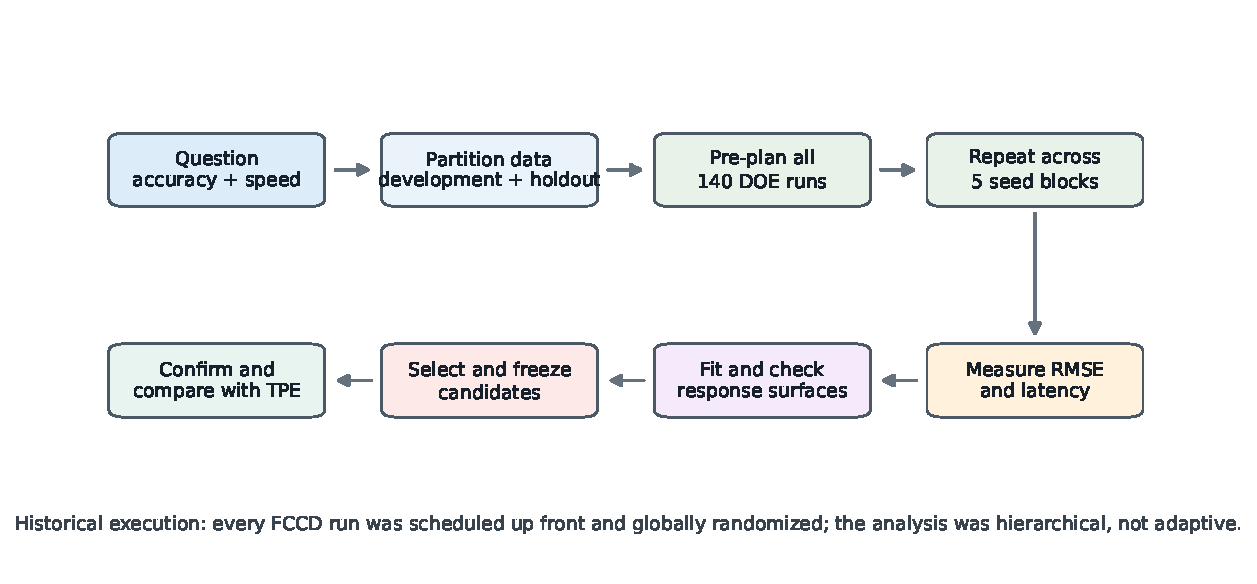
\includegraphics[width=\textwidth]{figures/explainer_research_pipeline.pdf}
\caption{The research pipeline. All \numPubDesignRuns{} historical FCCD runs were planned before execution and globally randomized. The labels ``Phase 1'' and ``Phase 2'' describe hierarchical analyses of that completed design; Phase 1 results did not decide whether later runs would be executed.}
\label{fig:pipeline}
\end{figure}

\section{Our core idea: learning from experiments}
An optimizer asks, ``Where should I try next to find a good model?'' A designed experiment also asks, ``What can this collection of trials teach us about the system?'' DOE chooses combinations so that changes in the response can be attributed to individual factors, interactions between factors, and curvature. \term{Response surface methodology (RSM)} then fits a low-order mathematical surface through those planned measurements \cite{box1951experimental,myers2016response}. The surface is a local guide: it can summarize broad tendencies and suggest candidates, but it must be checked against observations before being trusted.

We varied \numPubFactors{} XGBoost hyperparameters while holding the ensemble size at \numPubTrees{} trees:
\begin{table}[tbp]
\centering
\small
\renewcommand{\arraystretch}{1.2}
\begin{tabular}{p{0.21\textwidth}p{0.25\textwidth}p{0.18\textwidth}p{0.25\textwidth}}
\toprule
\textbf{Hyperparameter} & \textbf{Practical meaning} & \textbf{Studied range} & \textbf{Expected trade-off} \\
\midrule
Learning rate $\eta$ & Size of each boosting update & $\numPubEtaLow$--$\numPubEtaHigh$ (log scale) & Small values learn slowly; large values can converge faster but overshoot. \\
Maximum depth & Maximum tree complexity & \numPubDepthLow{}--\numPubDepthHigh{} & Deeper trees can model complex patterns but cost more to train and predict. \\
Subsample & Fraction of training rows used per tree & $\numPubSubLow$--$\numPubSubHigh$ & Sampling can regularize the model but adds stochastic variation. \\
$L_2$ regularization $\lambda$ & Penalty on leaf weights & $\numPubLambdaLow$--$\numPubLambdaHigh$ (log scale) & Stronger shrinkage can reduce overfitting but may suppress useful structure. \\
\bottomrule
\end{tabular}
\caption{The \numPubFactors{} studied factors. Log scaling gives multiplicative changes in learning rate and regularization comparable spacing in the experimental design.}
\label{tab:factors}
\end{table}

The face-centered central composite design (FCCD) combines factorial corners, axial points that move one factor at a time, and repeated center points. Figure~\ref{fig:design} shows a two-factor projection. Corners reveal main effects and interactions, axial points help estimate curvature, and center replicates measure variation when the nominal configuration is unchanged.
\begin{figure}[tbp]
\centering
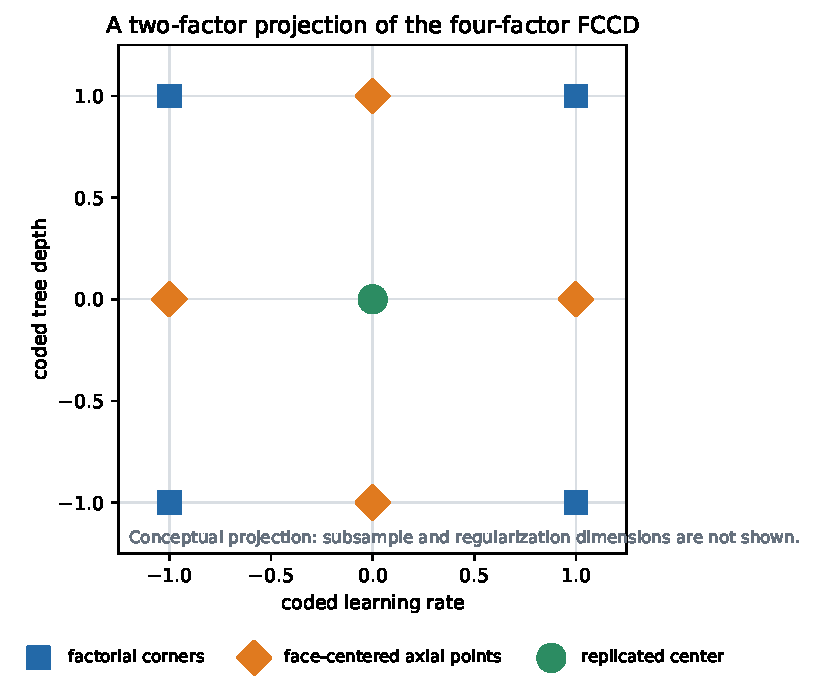
\includegraphics[width=0.69\textwidth]{figures/explainer_design_projection.pdf}
\caption{How the FCCD explores factor space. This simplified projection shows learning rate and depth only; the actual experiment used \numPubFactors{} dimensions. The same planned coordinate types were repeated across data-split blocks.}
\label{fig:design}
\end{figure}

\subsection{From a fixed design to an explanatory feedback loop}
The historical experiment was planned as a whole. The extension adds a genuinely sequential alternative: start with an informative design, fit models of the measured responses, use their uncertainty or disagreement to choose new configurations, and update the models after observing those configurations. This matters because an explanation is more useful when it helps us decide what to measure next, rather than merely describing an already completed search.

Figure~\ref{fig:extension} shows the implemented loop. Both the quadratic surface and the flexible model take hyperparameters as inputs and predict a measured outcome. ANOVA describes the fitted statistical effects; Shapley explanations describe contributions to a model's predictions. They examine the same response problem from different viewpoints, so agreement is an empirical question, not an assumption.
\begin{figure}[tbp]
\centering
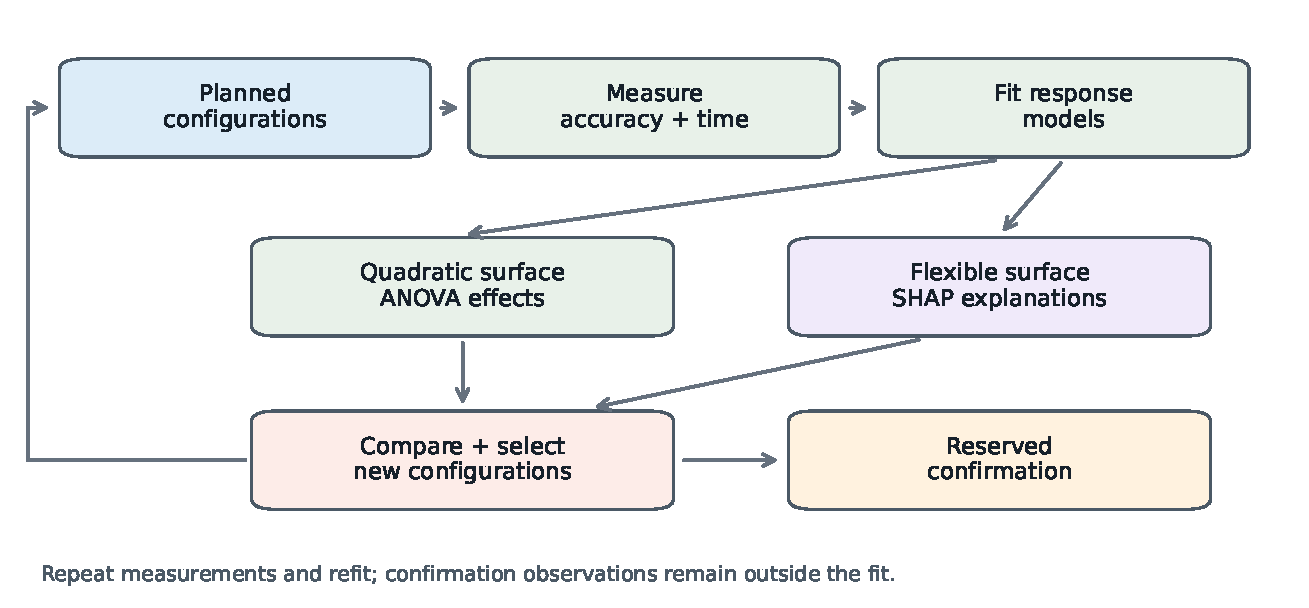
\includegraphics[width=\textwidth]{figures/explainer_sequential_extension.pdf}
\caption{The explainable sequential extension. Measured responses support statistical and flexible response models; their explanations and uncertainty guide additional experiments. Reserved confirmation observations check predictions without being used to fit these models. This diagram describes the implemented method, not a measured improvement over the housing results.}
\label{fig:extension}
\end{figure}

\section{How we designed the experiment}
\subsection{Data partitions and holdout history}
The California Housing dataset contains \numPubRows{} observations. A fixed \numPubHoldoutPct\% external holdout contained \numPubTestRows{} observations. The remaining \numPubDevRows{} observations formed the development pool. Within each seed block, that pool was divided into \numPubTrainRows{} training and \numPubValRows{} validation observations. Search decisions used validation RMSE, while final generalization checks used the holdout test set.

During the repeated benchmark experiments, the selection procedure programmatically prevented access to holdout outcomes until the models were fixed for final evaluation. Earlier experiments had already reported results from the same holdout dataset, however. The holdout therefore cannot be described as untouched across the project's full history.

\subsection{Why blocking was necessary}
Changing a hyperparameter is not the only reason RMSE changes. A different random split can make a training problem slightly easier or harder. We therefore repeated planned configurations across \numPubBlocks{} split seeds, called \term{blocks}. This allowed the statistical model to separate systematic hyperparameter effects from partition-related nuisance variation. Figure~\ref{fig:blocking} shows center-point observations: the configuration is nominally the same, yet the block means move.

The estimated block standard deviation was approximately \numSigmaBlock\ RMSE. Blocks accounted for an intraclass correlation of \numICCAnova\ (\numICCAnovaPct\ of unexplained residual variance), matching the REML estimate \numICCReml. This is not \numICCAnovaPct\ of total response variation; the main factor effects dominate the wide design region. It is nevertheless large enough to matter when competitive configurations differ by only a few thousandths of RMSE.
\begin{figure}[tbp]
\centering
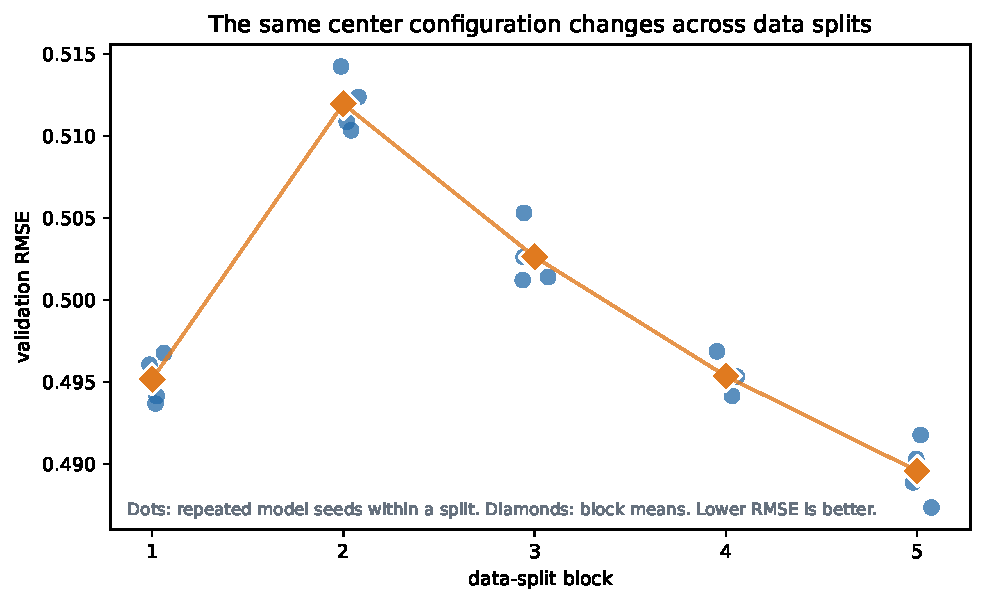
\includegraphics[width=0.72\textwidth]{figures/explainer_blocking.pdf}
\caption{Why blocking matters. Canonical center-point measurements vary across data-split blocks even though the hyperparameters remain fixed. Repeated model seeds within a block show subsampling variation; movement between block means shows partition variation.}
\label{fig:blocking}
\end{figure}

\subsection{What the \numPubDesignRuns{}-run design means}
Each of \numPubBlocks{} blocks contained \numPubCorners{} factorial corners, \numPubAxial{} face-centered axial points, and \numPubCenters{} center runs, giving \numPubDesignRuns{} model fits in total. All runs were generated in advance and globally randomized. In the shuffled execution order, \numDoeAxialBeforeHundred\ of the \numPubAxialTotal{} axial runs happened before run \numPubScreeningRuns{}. Thus the historical campaign was not an adaptive sequence in which an initial analysis triggered an augmentation.

The matched numerical budget needs qualification. DOE used \numPubCoordinates{} distinct coordinates across \numPubBlocks{} blocks plus extra center replication; TPE and Random Search used \numPubOptimizerTrials{} configuration evaluations on a fixed development split. DOE spent evaluations on variance estimation and structured effect identification. Adaptive search spent them on denser coordinate exploration. In addition, \numDoeLowEtaCount\ of the DOE's \numPubDesignRuns{} runs (\numDoeLowEtaPct) lay at $\eta=\numPubEtaLow$, where \numPubTrees{} trees underfit: mean validation RMSE was \numDoeLowEtaMeanRMSE\ there versus \numDoeHighEtaMeanRMSE\ elsewhere.

\subsection{What we measured}
For each trial we recorded development validation RMSE and single-row CPU prediction latency. The initial measurements used warmup and \numPubPrimaryCalls{} timed calls per prediction interface. The repeated searches used a cheaper \numPubOnlineCalls{}-call online measurement after \numPubOnlineWarmups{} warmup calls. Final benchmark verification used \numPubPrimarySessions{} separately randomized sessions under the warmed \numPubPrimaryCalls{}-call protocol. Standard \texttt{predict} also includes data-wrapper overhead: the interface comparison measured \numRevInterfaceOverhead\,$\pm$\,\numRevInterfaceOverheadSd\,$\mu$s more than \texttt{inplace\_predict}. Search-time latency and benchmark verification latency are therefore distinct measurements and are never treated as interchangeable.

\subsection{A separate sentiment-classification protocol}
The extension supports a researcher-supplied binary text-sentiment dataset, with an official test partition retained when available. It is a new application, rather than a reinterpretation of the housing measurements. Text is converted into sparse word and phrase features using TF--IDF, which gives more weight to informative expressions. Each development fold learns its vocabulary and feature weights from its training documents only; its validation documents do not influence preprocessing.

Accuracy is measured with macro-averaged F-score, which gives the sentiment classes equal weight, and log loss, which also assesses predicted probabilities. The optimization loss is the complement of macro F-score, so smaller remains better. Prediction time is measured for an individual document. The factors retain learning rate, depth, and row subsampling; feature subsampling replaces the housing study's leaf-weight regularization factor. This change is appropriate to a sparse text representation but prevents treating the experiments as direct replications.

The learning-rate domain excludes the housing study's severe underfitting setting. This is a design precaution, not evidence that underfitting disappears on text. Model capacity, factor ranges, and the operational latency limit still need development-only calibration for the chosen dataset. The new timing operation uses a fresh prediction input wrapper for each classic-API call, alongside a separately recorded in-place operation, with the same warmed protocol throughout the new study. Their different input-conversion costs are explicitly retained.

\section{How we learned from the experimental results}
\subsection{Screening and curvature}
The first analysis asked which effects were large enough to deserve attention. Learning rate dominated the first-order factorial model ($F=\numAnovaPOneFxone$), followed by depth ($F=\numAnovaPOneFxtwo$) and their interaction ($F=\numAnovaPOneFxoneXtwo$). An interaction means the effect of one setting depends on another: increasing depth does not have one constant consequence at every learning rate.

Center runs then tested whether a flat plane was adequate. The factorial mean exceeded the center mean by \numDiffCurv\ RMSE (\numCurvPctIncrease). Curvature was strong under every reported error denominator: $F=\numFCurv$ against center pure error, $F=\numCurvFBlockAdjPooled$ against pooled block-adjusted error, and $F=\numCurvFBlockPaired$ in the paired \numPubBlocks{}-block analysis. The conclusion is non-planarity, not proof that a quadratic surface is globally correct. That distinction motivated the second-order fit and its adequacy tests.

\subsection{How settings shaped accuracy}
We wanted a mathematical picture of how learning rate and tree depth changed accuracy, rather than only a ranked list of configurations. Figure~\ref{fig:surface-rmse} shows a two-factor slice of the fitted quadratic surface. The horizontal axis is coded log learning rate, the vertical axis is coded maximum depth, and the contours and height show predicted validation RMSE; darker, lower regions are better. The surface falls sharply as learning rate moves away from the underfitting boundary, then forms a broad ridge. The cyan depth-\numPubDepthSo{} candidate sits near the best in-domain region, while the stationary point indicated by the arrow lies outside the experimental domain. This geometry is why we optimized within the tested bounds and required confirmation.
\begin{figure}[H]
\centering
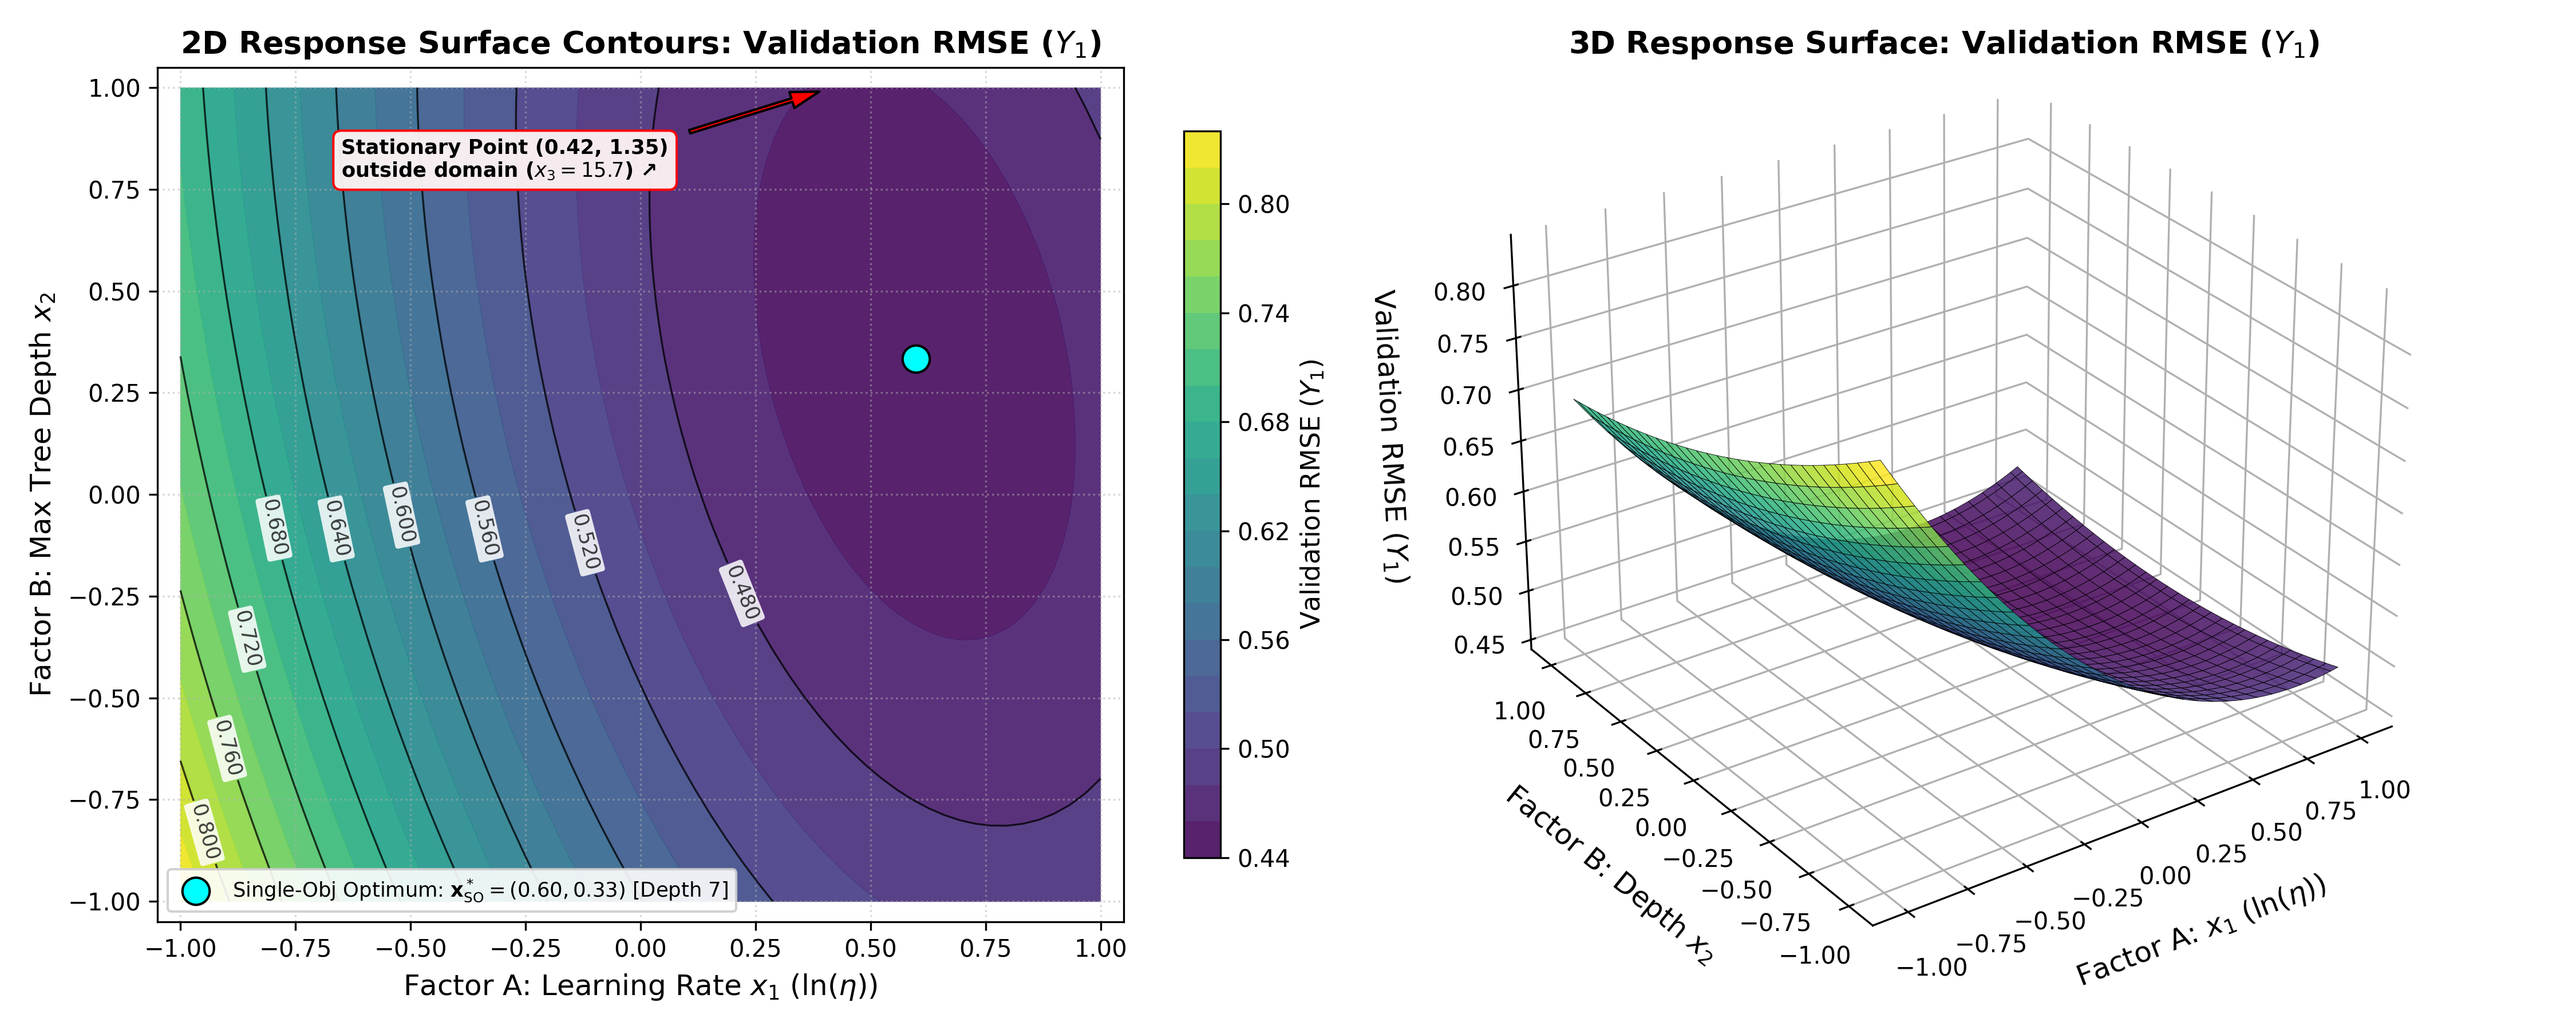
\includegraphics[width=\textwidth]{figures/response_surface_rmse_2d_3d.png}
\caption{Empirical validation-RMSE response surface. Left: contours across coded log learning rate and depth at the single-objective slice. Right: the same fitted surface in three dimensions. The broad valley guides candidate selection, but the extrapolated stationary point lies outside the studied region.}
\label{fig:surface-rmse}
\end{figure}

The quadratic validation-RMSE model had $R^2=\numRsqRMSE$ and adjusted $R^2=\numAdjRsqRMSE$. These high values mainly reflect large changes across the full learning-rate range. Formal lack-of-fit remained significant: $F=\numFLofYone$ with $p=\numPLofYone$, and the lack-of-fit RMS scale was \numSqrtMSLofYone. When the severe $\eta=\numPubEtaLow$ boundary was removed, lack-of-fit sum of squares fell by \numLofRestrictedReductionPct, although the restricted model still did not justify treating the surface as exact.

The residual diagnostics, reproduced in the technical supplement, showed approximately normal residuals but also heteroscedasticity and localized influence. HC3 heteroscedasticity-consistent standard errors were used separately for coefficient inference; they do not remove model misspecification. Breusch--Pagan provided evidence of heteroscedasticity, while the serial diagnostics did not detect significant dependence in the tested residual order. Those diagnostics do not prove the absence of every temporal pattern or independently establish the absence of thermal drift.

\subsection{How model complexity affected speed}
The next question was whether deeper trees imposed a predictable latency cost. In Figure~\ref{fig:latency-depth}, the horizontal axis is maximum tree depth and the vertical axis is measured single-sample prediction time. The left panel compares empirical means and \numPubCoveragePct\% intervals with linear and quadratic fits; the right panel shows the full distribution at each tested depth. Latency rises modestly from depth \numPubDepthLow{} to \numPubDepthMiddle{} and much more sharply by depth \numPubDepthHigh{}, so a straight line understates the acceleration.
\begin{figure}[H]
\centering
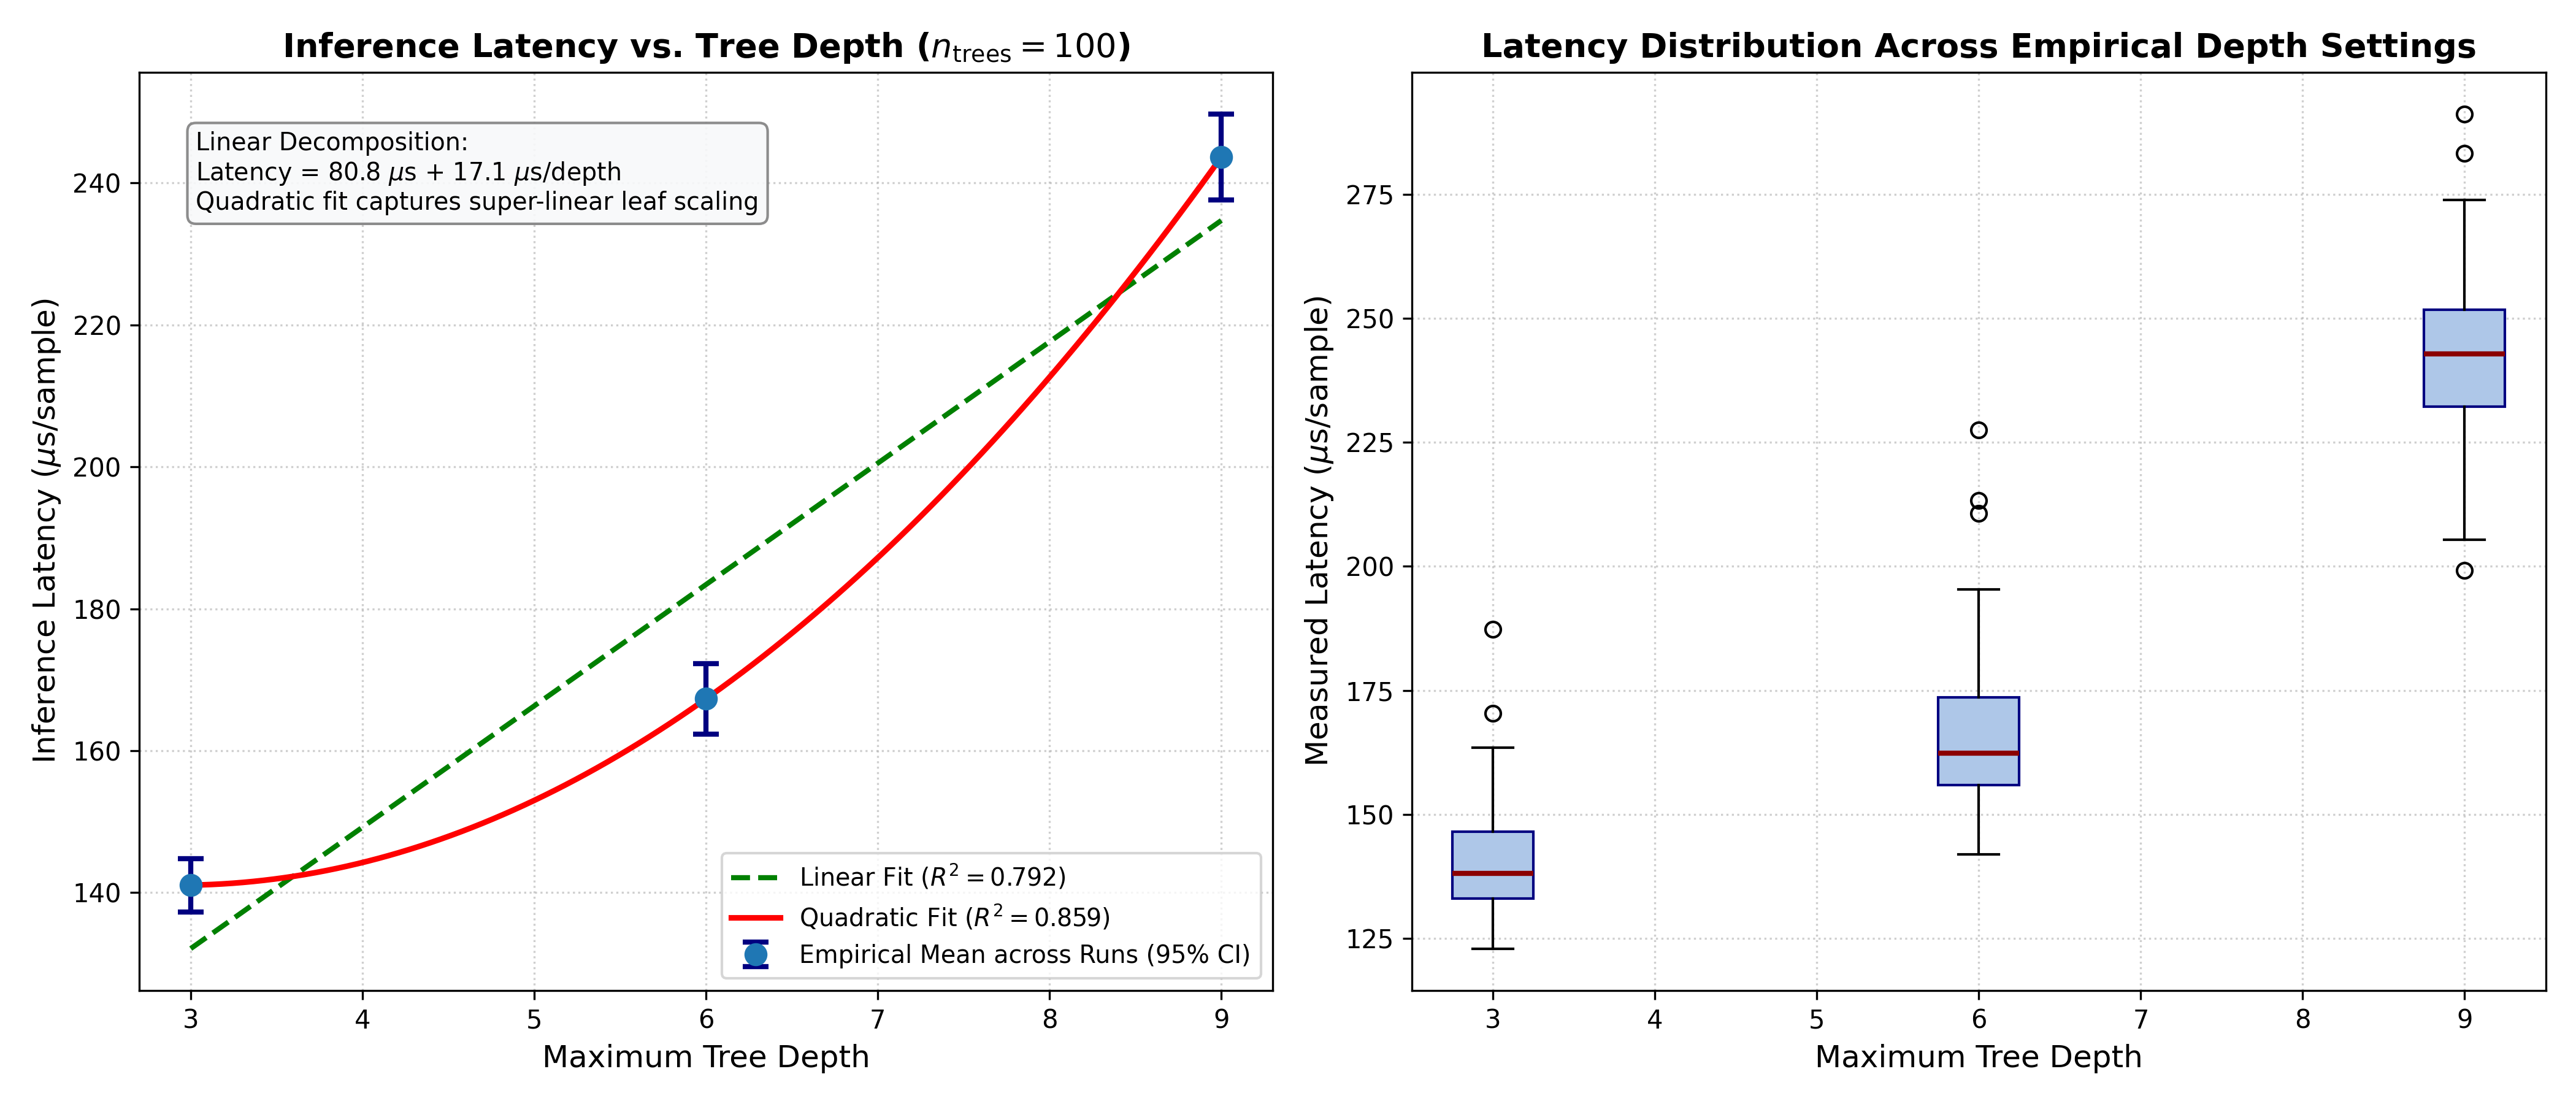
\includegraphics[width=\textwidth]{figures/response_surface_latency_2d_3d.png}
\caption{Measured prediction latency by maximum tree depth. The quadratic curve follows the accelerating cost better than the linear fit, while the boxplots show run-to-run variation around each tested depth.}
\label{fig:latency-depth}
\end{figure}

A quadratic depth profile achieved $R^2=\numLatQuadRsq$ compared with $R^2=\numLatLinRsq$ for a linear profile. Latency lack of fit was not significant ($F=\numFLofYtwo$, $p=\numPLofYtwo$). This result applies to the tested hardware and single-sample protocol, not to batch throughput or all deployment systems. The observed acceleration made depth central to the later accuracy--speed compromise.

\subsection{Comparing statistical effects with model explanations}
The extension asks whether the settings highlighted by ANOVA also matter to a flexible predictor of the measured response. A Gaussian process provides an alternative to the quadratic surface: it can represent smooth nonlinear patterns and supplies model-based prediction uncertainty. It must earn our trust through new observations, just as the polynomial must.

Shapley explanations distribute a prediction's departure from a background prediction among its input settings \cite{lundberg2017unified}. Pairwise interaction values ask how the contribution of settings considered together differs from their separate contributions. The implementation evaluates the complete coalition calculation over the recorded experimental background; multiplying ordinary attribution scores is not used as an interaction measure.

Here, the explained inputs are hyperparameters, not words in a review. Explaining which words caused a sentiment decision would be a separate analysis of the classifier itself. Keeping these levels distinct lets us ask the intended question: which settings control accuracy and speed, and when does the fitted response model regard their effects as interdependent?

We compare factor rankings, pairwise interaction patterns, and main-effect dependence profiles. Curved dependence suggests that a setting's effect changes across its range. ANOVA sums of squares and Shapley contributions have different meanings and units, however; correlation is descriptive agreement, not mathematical equivalence. Undefined correlations stay undefined. Comparisons across development blocks and before and after augmentation can reveal which explanations are stable and where more evidence is needed. No real sentiment-data result for these comparisons is claimed here.

\section{How we selected candidate models}
The fitted surface had a nearly flat direction: its smallest canonical eigenvalue was \numEigOne, with bootstrap interval $[\numBootLowEigOne,\numBootHighEigOne]$, and \numFracMinEigLeZero\ of bootstrap replicates placed it at or below zero. The unconstrained stationary point lay far outside the studied region. We therefore interpret the geometry as a stationary or rising ridge rather than a well-defined bowl with one stable interior minimum.

We used two selection goals. The \term{single-objective} candidate minimized predicted validation RMSE and moved toward a depth-\numPubDepthSo{} boundary solution. The \term{multi-objective} candidate combined RMSE and latency through a Derringer--Suich desirability score \cite{derringer1980simultaneous}: each outcome was converted to a preference between zero and one, then combined. This selected an interior depth-\numPubDepthMo{} compromise with learning rate \numOptEta, subsample \numOptSubsample, regularization \numOptLambda, and composite desirability \numOptD.

Figure~\ref{fig:desirability-pareto} shows how that decision emerged from the planned experiment. The horizontal axis is \numPubBlocks{}-block mean validation RMSE and the vertical axis is \numPubBlocks{}-block mean latency; moving left or down is better. Pale points are individual block observations, colored circles are configuration means, and the dashed staircase is the observed Pareto front. A point is \term{Pareto efficient} when no observed alternative is better on both outcomes. The depth-\numPubDepthSo{} diamond pursues accuracy, whereas the depth-\numPubDepthMo{} star gives up a small amount of predicted accuracy for much lower latency. That trade-off motivated carrying both candidates into confirmation.
\begin{figure}[H]
\centering
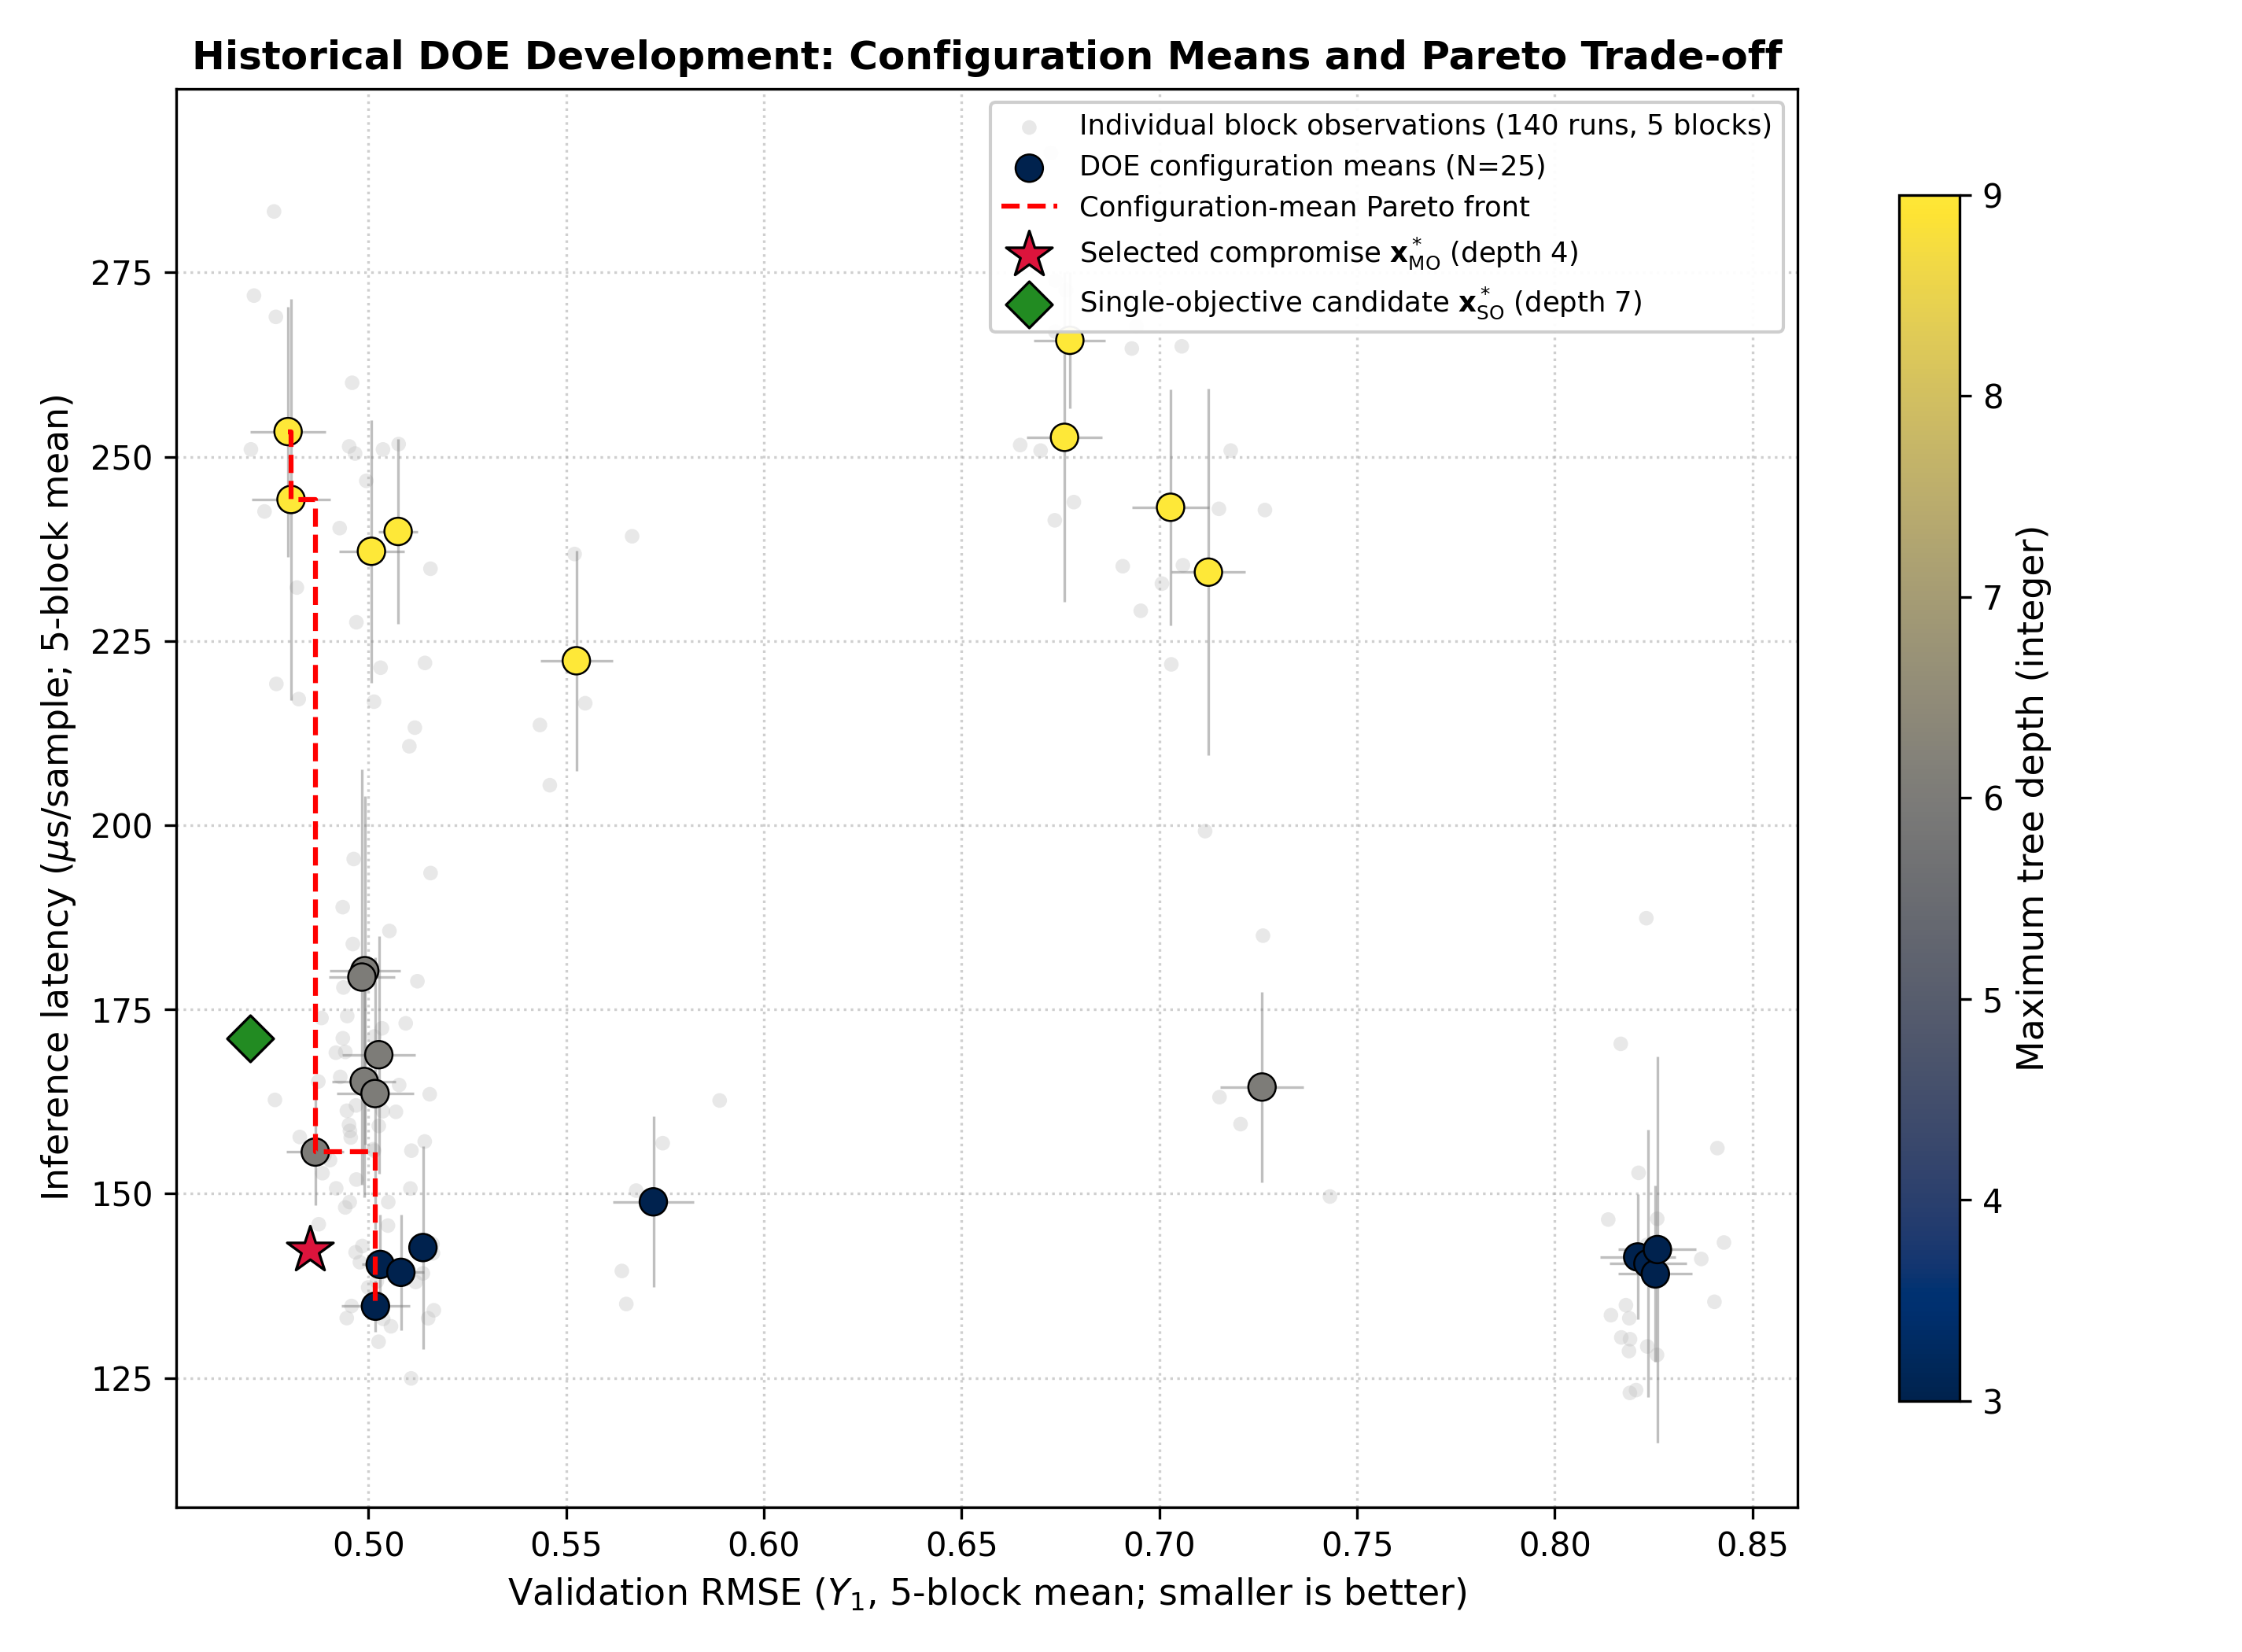
\includegraphics[width=0.82\textwidth]{figures/desirability_pareto_front.png}
\caption{Accuracy--speed evidence from the initial blocked experiment. Configuration means and their between-block uncertainty reveal the Pareto trade-off used to select the depth-\numPubDepthMo{} compromise and depth-\numPubDepthSo{} accuracy candidate.}
\label{fig:desirability-pareto}
\end{figure}

Sensitivity analysis changed desirability bounds and weights. The compromise moved as intended rather than producing one invariant optimum, which is why the desirability choice is treated as a declared decision rule rather than a discovered physical constant. Full sensitivity results remain in the technical supplement.

\subsection{Choosing genuinely new evaluations}
In the extension, new configurations can target uncertain predictions, disagreement between the quadratic and flexible models, or a mixture of uncertainty and space coverage. A further option favors expected improvement in a declared normalized accuracy--latency score. This is scalarized improvement, not expected improvement of Pareto hypervolume. The score and its incumbent use the same block-averaged response, avoiding comparison with an unusually favorable individual split.

Tree depth is treated as an integer before a point is scored, checked for duplication, trained, or logged. Otherwise, the response model could learn from a fractional setting that was never executed. Each adaptive batch is measured across the development blocks before refitting. Reserved confirmation configurations are excluded from the fitting and acquisition evidence.

\section{How we checked whether the findings held up}
First, we evaluated the historical candidates across ten confirmation seeds:
\[
\mathcal{S}_{\text{conf}}=\{\numPubConfirmationSeeds\}.
\]
The intervals combined regression uncertainty with estimated block variance through a Satterthwaite approximation. This reflects uncertainty from a new partition, but it cannot guarantee protection against localized polynomial bias.
\begin{table}[tbp]
\centering
\small
\setlength{\tabcolsep}{3.2pt}
\begin{tabular}{lcccc}
\toprule
\makecell[l]{\textbf{Configuration /}\\\textbf{Response Metric}} & \makecell{\textbf{Surrogate}\\\textbf{Pred ($\hat{y}$)}} & \makecell{\textbf{95\% Pred}\\\textbf{Interval (PI)}} & \makecell{\textbf{Empirical}\\\textbf{Mean $\pm$ SD}} & \makecell{\textbf{Confirmation}\\\textbf{Status}} \\
\midrule
\multicolumn{5}{l}{\textbf{DOE Multi-Objective Optimum $\mathbf{x}^*_{\text{MO}}$ (Depth 4)}} \\
Validation RMSE ($Y_1$) & $0.4804$ & $[0.4677, 0.4932]$ & $0.4853 \pm 0.0115$ & \makecell[c]{\textbf{Pass}\\(Inside 95\% PI)} \\
Holdout Test RMSE & --- & --- & $0.4888 \pm 0.0032$ & Holdout Test Set \\
Inference Latency ($\mu$s) & $138.1$ & $[122.8, 153.4]$ & $142.3 \pm 7.8$ & \makecell[c]{\textbf{Pass}\\(Inside 95\% PI)} \\
\midrule
\multicolumn{5}{l}{\textbf{DOE Single-Objective Candidate $\mathbf{x}^*_{\text{SO}}$ (Depth 7)}} \\
Validation RMSE ($Y_1$) & $0.4483$ & $[0.4354, 0.4612]$ & $0.4700 \pm 0.0093$ & \makecell[c]{\textbf{Not Confirmed}\\(Optimism: +0.0217)} \\
Holdout Test RMSE & --- & --- & $0.4691 \pm 0.0034$ & Holdout Test Set \\
Inference Latency ($\mu$s) & $187.0$ & $[171.1, 202.9]$ & $171.1 \pm 10.9$ & \makecell[c]{Borderline\\(At Lower PI)} \\
\bottomrule
\end{tabular}

\caption{Independent confirmation of the historical multi-objective compromise and accuracy-focused boundary candidate. The compromise confirmed within its interval; the boundary candidate exposed polynomial optimism.}
\label{tab:confirmation}
\end{table}

The depth-\numPubDepthMo{} compromise produced validation RMSE \numConfEmpValRMSE\,$\pm$\,\numConfEmpValRMSEStd, inside its \numPubCoveragePct\% interval $[\numConfPiLowValRMSE,\numConfPiHighValRMSE]$. The depth-\numPubDepthSo{} candidate produced \numConfSoEmpValRMSE\,$\pm$\,\numConfSoEmpValRMSEStd, above its upper interval bound by \numConfSoExceedance\ and showing optimism bias \numConfSoBias. Confirmation therefore supported the compromise pointwise while warning against global trust in the surface.

For the repeated benchmark experiments, every selected configuration was fixed before final evaluation. Each selection was then retrained across \numPubEvalSeeds{} seeds from \numPubFirstEvalSeed{} through \numPubLastEvalSeed{} and assessed on the external holdout. Repeated DOE used \numPubSearchReplicates{} fresh search replicates, each containing \numPubRepeatedBlocks{} development blocks. Its single-objective rule selected the same predeclared grid point in every replicate, so between-search SD was \numRevDoeSoTestRMSESd; conditional retraining SD at that configuration was still \numRevDoeSoRetrainSd. These quantities describe different sources of variation and must not be conflated.

\subsection{Confirmation for the sequential extension}
The new protocol separates three questions. New configurations in the existing development blocks test whether the response models predict beyond their fitting points. Comparisons of the polynomial and Gaussian-process errors test whether extra flexibility improves approximation. Final test observations assess the selected classifier after its choice has been fixed.

For the quadratic extension model, intervals use ordinary fixed-block regression. They predict observations in known blocks; without a specified block, the interval describes the adjusted mean across observed blocks. They are not the historical Satterthwaite intervals and do not promise prediction for an unseen stochastic block. Gaussian-process intervals are model-based and are checked separately. Coverage, prediction error, and boundary bias therefore remain measured diagnostics, not guarantees supplied by the model name.

Final test access is gated by frozen selections. The final vocabulary is then learned from the development pool, and the reserved test data are evaluated under that fixed choice. This procedure protects selection within the new experiment; it cannot demonstrate that a supplied dataset was never examined previously. Dataset identity and prior exposure must still be assessed scientifically.

\clearpage
\section{Comparing DOE with alternative optimization methods}
We compared the following adaptive or stochastic alternatives:
\begin{itemize}
\item \term{Random Search} samples configurations without learning from earlier results.
\item \term{Single-Objective TPE} adapts its sampling to reduce validation RMSE.
\item \term{Multi-Objective TPE} searches for configurations spanning the RMSE--latency trade-off.
\item \term{Constrained TPE} minimizes RMSE while treating \numPubLatencyLimit\,$\mu$s as a latency constraint.
\end{itemize}

Table~\ref{tab:methods} explains why equal counts of model fits do not make the information identical. The complete campaign used \numRevTotalFits\ model fits. Each search replicate used \numPubSearchFits{} fits, but DOE replicated planned coordinates across splits while black-box methods allocated trials to coordinate exploration on a fixed split. The technical supplement provides the detailed execution budget and timing ledger.
\begin{table}[H]
\centering
\small
\setlength{\tabcolsep}{5pt}
\renewcommand{\arraystretch}{1.3}
\begin{tabularx}{\textwidth}{@{}>{\raggedright\arraybackslash}p{0.15\textwidth}>{\raggedright\arraybackslash}p{0.23\textwidth}>{\raggedright\arraybackslash}p{0.20\textwidth}>{\raggedright\arraybackslash}X@{}}
\toprule
\textbf{Method} & \textbf{Use of the \numPubSearchFits{}-fit budget} & \textbf{Noise handling during search} & \textbf{Primary information gained} \\
\midrule
Blocked DOE & \numPubCoordinates{} planned coordinates & \numPubRepeatedBlocks{} data-split blocks & Effects, interactions, curvature, and split-to-split variation \\
Random Search & \numPubOptimizerTrials{} sampled trials & Fixed development split & Broad non-adaptive exploration \\
TPE variants & \numPubOptimizerTrials{} adaptive trials & Fixed development split & Concentrated optimization in promising regions \\
\bottomrule
\end{tabularx}
\caption{What the compared methods did with the same \numPubSearchFits{}-fit search budget. DOE emphasized estimable effects and split-to-split variation; Random Search emphasized broad coverage; TPE emphasized adaptive concentration. These are different experimental estimands even when fit counts match. Each search was repeated \numPubSearchReplicates{} times, and fixed selections were retrained across \numPubEvalSeeds{} evaluation seeds.}
\label{tab:methods}
\end{table}

Figure~\ref{fig:efficiency} retains the archived trajectories to show what was recorded during the historical searches. Its horizontal axis counts model fits and its vertical axis shows the lowest logged validation RMSE so far. For TPE on a fixed split, a falling curve describes improvement in that split's objective. The DOE trace instead combines observations from different validation blocks: its running minimum favors whichever block happens to be easier and is not the block-adjusted candidate-selection rule. The curves therefore cannot establish a controlled ranking of search efficiency. This limitation motivates the shared-block comparison in the sequential extension.
\begin{figure}[H]
\centering
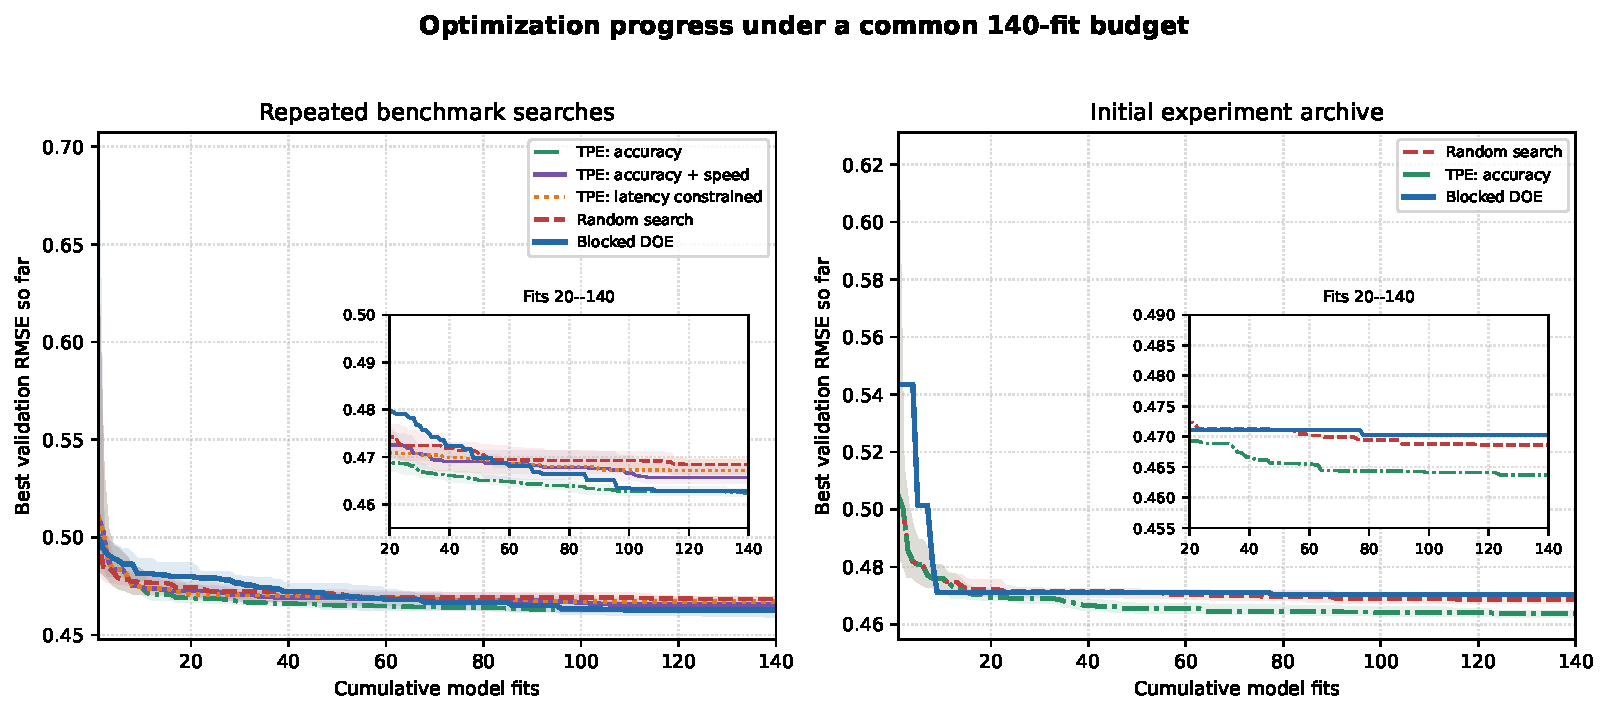
\includegraphics[width=\textwidth]{figures/explainer_efficiency_comparison.pdf}
\caption{Archived running minima under the historical \numPubSearchFits{}-fit budget. DOE mixes validation blocks and does not represent a common-estimand incumbent curve. Left: medians and interquartile bands from \numPubSearchReplicates{} repeated searches per method. Right: the initial single planned experiment compared with archived random-search and TPE trajectories. Lower curves are better; the insets magnify later differences.}
\label{fig:efficiency}
\end{figure}

\begin{table}[tbp]
\centering
\scriptsize
\setlength{\tabcolsep}{2.5pt}
\resizebox{\textwidth}{!}{\begin{tabular}{lcccccc}
\toprule
\makecell{\textbf{Optimization}\\\textbf{Method}} & \makecell{\textbf{Search Basis}\\\scriptsize($N$ Reps)} & \makecell{\textbf{Val RMSE}\\\scriptsize Mean $\pm$ SD} & \makecell{\textbf{Holdout}\\\textbf{Test RMSE}\\\scriptsize Mean $\pm$ SD} & \makecell{\textbf{Retrain}\\\bm{$\sigma_{\text{eval}}$}} & \makecell{\textbf{Latency}\\\scriptsize($\mu\text{s} \pm \text{SD}$)} & \makecell{\textbf{Feasible}\\\scriptsize($\le 145\,\mu\text{s}$)} \\
\midrule
\multicolumn{7}{l}{\textbf{Panel A: Repeated Benchmark Experiments ($N=20$ Search Replicates)}} \\
\makecell[l]{Repeated DOE MO\\($\mathbf{x}^*_{\text{MO}}$)} & RSM ($N{=}20$) & $0.4853 \pm 0.0055$ & $0.4900 \pm 0.0073$ & $0.0033$ & $122.3 \pm 2.7$ & 20/20 \\
\makecell[l]{Multi-Objective TPE} & Parzen ($N{=}20$) & $0.4881 \pm 0.0093$ & $0.4926 \pm 0.0108$ & $0.0036$ & $121.5 \pm 3.8$ & 20/20 \\
\makecell[l]{Constrained TPE\\($\le 145\,\mu\text{s}$)} & Parzen ($N{=}20$) & $0.4700 \pm 0.0022$ & $0.4704 \pm 0.0032$ & $0.0034$ & $144.3 \pm 7.1$ & 9/20 \\
\makecell[l]{Repeated DOE SO\\($d{=}7$)} & RSM ($N{=}20$) & $0.4687 \pm 0.0000$ & $0.4686 \pm 0.0000$ & $0.0030$ & $150.7 \pm 0.7$ & 0/20 \\
\makecell[l]{Single-Objective TPE} & Parzen ($N{=}20$) & $0.4675 \pm 0.0008$ & $0.4669 \pm 0.0012$ & $0.0031$ & $188.9 \pm 12.1$ & 0/20 \\
\makecell[l]{Unguided Random Search} & Uniform ($N{=}20$) & $0.4687 \pm 0.0014$ & $0.4695 \pm 0.0021$ & $0.0030$ & $181.1 \pm 19.0$ & 0/20 \\
\midrule
\multicolumn{7}{l}{\textbf{Panel B: Initial Experiment Snapshot (Single Search Replicate)}} \\
\makecell[l]{Historical DOE MO\\($\mathbf{x}^*_{\text{MO}}$)} & RSM (Single) & $0.4821$ & $0.4884$ & --- & $119.8$ & Yes \\
\makecell[l]{Historical Multi-Obj TPE} & Parzen (Single) & $0.4812$ & $0.4870$ & --- & $118.8$ & Yes \\
\makecell[l]{Historical Constrained TPE} & Parzen (Single) & $0.4783$ & $0.4823$ & --- & $125.4$ & Yes \\
\makecell[l]{Historical DOE SO\\($d{=}7$)} & RSM (Single) & $0.4687$ & $0.4690$ & --- & $147.8$ & No \\
\makecell[l]{Historical Bayesian TPE} & Parzen (Single) & $0.4735$ & $0.4726$ & --- & $193.2$ & No \\
\makecell[l]{Historical Random Search} & Uniform (Single) & $0.4696$ & $0.4707$ & --- & $198.1$ & No \\
\bottomrule
\end{tabular}
}
\caption{Final benchmark results across \numPubSearchReplicates{} repeated searches and \numPubEvalSeeds{} holdout retraining seeds. Initial single-campaign rows are retained for context and are not interchangeable with the repeated benchmark experiments.}
\label{tab:benchmarks}
\end{table}

\begin{sloppypar}
Single-objective TPE achieved the lowest observed mean holdout RMSE, \numRevSoTpeTestRMSE\,$\pm$\,\numRevSoTpeTestRMSESd, at \numRevSoTpePredictLat\,$\pm$\,\numRevSoTpePredictLatSd\,$\mu$s. Repeated DOE single-objective achieved \numRevDoeSoTestRMSE\ at \numRevDoeSoPredictLat\,$\mu$s, which was \numRevDoeSoLatLowerPct\ lower latency. Neither accuracy-only method satisfied the latency constraint.

For multi-objective selection, Repeated DOE achieved \numRevDoeMoTestRMSE\,$\pm$\,\numRevDoeMoTestRMSESd\ RMSE at \numRevDoeMoPredictLat\,$\mu$s; multi-objective TPE achieved \numRevMoTpeTestRMSE\,$\pm$\,\numRevMoTpeTestRMSESd\ at \numRevMoTpePredictLat\,$\mu$s. The primary unpaired Welch comparison gave $\Delta=\numRevDiffDoeMoMoTpe$, $t=\numRevWelchTDoeMoMoTpe$, and $p=\numRevWelchPDoeMoMoTpe$. Replicate indices did not share a random block, so an index-paired result is only a secondary sensitivity check. No equivalence margin was pre-registered: failure to detect a difference is not evidence of equivalence.

Constrained TPE appeared feasible in \numRevCtpeSearchFeas\ online searches but only \numRevCtpeBenchFeas\ (\numRevCtpeBenchFeasPct) remained feasible under warmed \numPubPrimaryCalls{}-call verification. Depth-\numPubCtpeShallow{} selections were feasible at \numRevCtpeDepthSixLat\,$\mu$s; depth-\numPubCtpeDeep{} selections were not, averaging \numRevCtpeDepthSevenLat\,$\mu$s. Short noisy timing, protocol differences, and selection near the threshold are plausible explanations.
\end{sloppypar}

The final question was what the competing selected models achieved after retraining. In Figure~\ref{fig:pareto}, the left panel plots search-time validation RMSE against online latency for development candidates; the right plots holdout RMSE against verified latency for the fixed selections. Horizontal and vertical uncertainty bars on the right show retraining and timing variation. The red dashed frontier identifies choices for which no tested alternative was both more accurate and faster.

On development split \numPubDevelopmentSeed{}, multi-objective TPE candidate fronts had mean hypervolume \numRevHvMoTpeDevMean\,$\pm$\,\numRevHvMoTpeDevSd\ at reference $[\numPubHvPrimaryLoss, \numPubHvPrimaryTime]$, compared with \numRevHvDoeDevMean\,$\pm$\,\numRevHvDoeDevSd\ for \numPubBlocks{}-block repeated DOE means and \numRevHvFullDoeDev\ for the fixed \numPubFullFrontCount{}-point DOE front. These rows use different candidate pools and timing protocols. On the holdout, \numRevHoldoutNonDominatedConfigs\ distinct configurations formed the non-dominated set with frozen hypervolume \numRevHvHoldoutFrozen; seed-bootstrap mean was \numRevHvHoldoutBootSeedMean\ with \numPubCoveragePct\% interval $[\numRevHvHoldoutBootSeedCiLow,\numRevHvHoldoutBootSeedCiHigh]$. The secondary reference point was $[\numPubHvSecondaryLoss, \numPubHvSecondaryTime]$.
\begin{figure}[H]
\centering
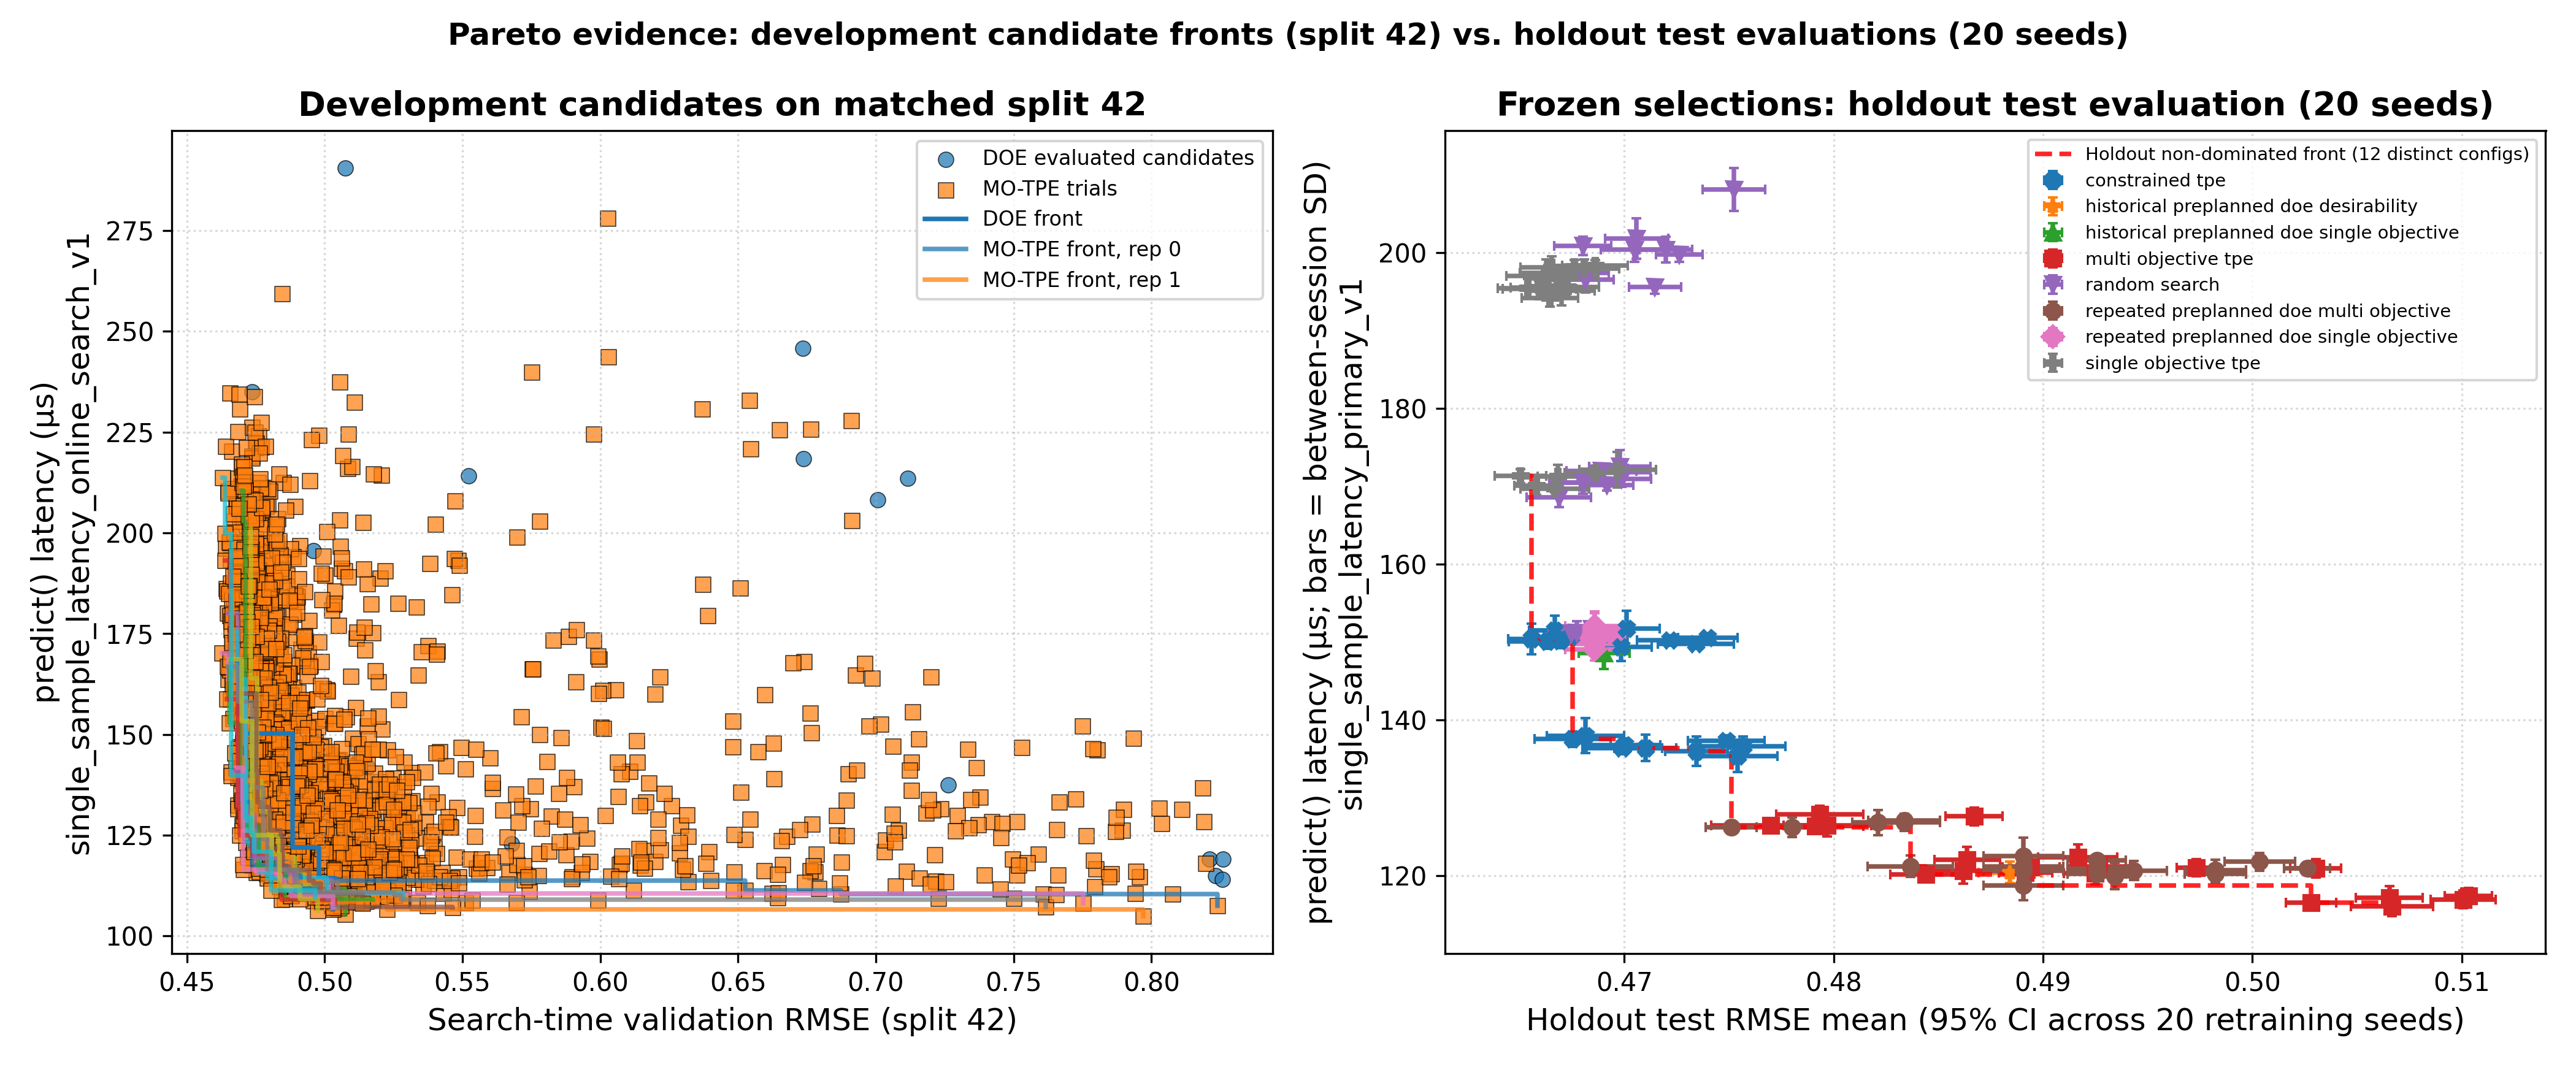
\includegraphics[width=0.92\textwidth]{figures/revision_v2_pareto_front.png}
\caption{Canonical Pareto evidence. Left: development candidate fronts under their stated search protocols. Right: frozen selections after independent holdout evaluation, including uncertainty. The figure separates development search measurements from final benchmark measurements.}
\label{fig:pareto}
\end{figure}

\subsection{A comparison with shared information}
The sequential extension gives DOE and multi-objective TPE the same development partitions, tree count, candidate-response aggregation, and inference operation. Every proposed configuration is evaluated across all development blocks, and the budget counts real classifier fits, including initial and adaptive design evaluations. Reserved confirmation and final evaluation are accounted for separately, so neither method receives hidden search evaluations.

The comparison records validation Pareto quality, the observed feasible fraction, optimizer overhead, and variability across repeated searches. Its regret summary refers to the best configuration observed by the compared methods, not the unknown global optimum. Final test observations remain separate from validation fronts. These distinctions let us interpret whether any advantage comes from search, explanation, replication, or the measurement protocol.

The available text workflow evidence is synthetic and demonstrates execution and separation of stages only. It cannot answer which method is better on a real sentiment dataset, whether interaction rankings generalize, or whether the new intervals have adequate real-data coverage. Those results require the separately specified sentiment study. The housing tables and graphs above remain the empirical findings of this report.

\section{What we learned}
\begin{enumerate}[leftmargin=1.6em,itemsep=0.45em]
\item \textbf{Structured DOE explains variation well.} It identified dominant factors and interactions, quantified curvature, and separated an estimated split-related nuisance component from treatment effects.
\item \textbf{A response surface is a guide, not ground truth.} Strong global $R^2$ coexisted with significant local lack of fit and a failed confirmation interval at the boundary candidate.
\item \textbf{Adaptive search used the budget effectively for point optimization.} Single-objective TPE found the lowest observed RMSE, and multi-objective TPE produced strong development fronts by concentrating trials in promising regions.
\item \textbf{The deployment choice depends on the accuracy--speed objective.} The fastest acceptable and most accurate configurations were different; the holdout frontier contained selections from DOE and several TPE variants.
\item \textbf{Latency constraints require careful verification.} Constrained TPE's feasibility dropped from search to warmed benchmarking, showing that a noisy online timing estimate is insufficient near a hard threshold.
\item \textbf{The comparison remains limited.} DOE and TPE used equal fit counts but different coordinate replication, split structures, and timing protocols. The fixed holdout does not estimate dataset-sampling uncertainty, and prior historical exposure prevents describing it as untouched. Results come from one dataset, one hardware environment, \numPubFactors{} factors, and \numPubTrees{} trees. Stronger claims require fresh outer test splits or additional datasets, matched timing protocols, more model families, and designs that include the number of trees.
\end{enumerate}

The extension turns these lessons into a testable scientific method: compare explanations of the same measured response, direct additional experiments toward uncertainty or disagreement, and check predictions on reserved configurations. Its value is the explicit connection between explanation, experimental choice, and confirmation. Whether it improves accuracy--speed trade-offs or explanation stability on text remains an open empirical question.

\section{Conclusion}
A pre-planned blocked experiment can do more than produce a candidate configuration: it can show which hyperparameters matter, expose interactions and curvature, quantify random split effects, and reveal when its own approximation is inadequate. In this study, that explanatory value coexisted with clear limitations. The quadratic surface was not globally faithful, the accuracy-focused DOE candidate was optimistic in confirmation, and adaptive TPE found the lowest observed single-objective RMSE.

The multi-objective evidence does not identify one universal winner. Repeated DOE and multi-objective TPE produced similar observed holdout performance at comparable latency, with no statistically significant detected difference and no basis for an equivalence claim. The practical lesson is to combine the strengths of both approaches: use structured experiments when explanation, variance decomposition, and stable comparison matter; use adaptive search when dense exploitation of promising regions is the main goal; and independently confirm every selected model under the deployment measurement protocol.

The implemented sequential extension provides the next test of that complementary approach. It joins statistical effect analysis, flexible response modeling, Shapley interaction explanations, adaptive acquisition, and protected final evaluation. It does not convert the completed housing experiment into a sequential one or establish new sentiment-performance results. The next scientific decision is to select and calibrate a fresh text study, then judge the method from its independent observations rather than from its implementation alone.

\section{Code availability}
The code and research materials are publicly available at: \url{https://github.com/ChristosHussein/xgboost-doe-rsm}

\section*{Companion technical supplement}
The complete derivations, generated ANOVA and adequacy tables, residual diagnostics, timing forensics, hypervolume details, computational budget, and claim-level provenance are provided in \texttt{technical\_supplement.pdf}. The comprehensive numerical record remains in \texttt{REPORT.md}.

\clearpage
\begin{thebibliography}{9}
\small
\setlength{\itemsep}{0pt}
\bibitem{montgomery2017design} D.~C. Montgomery, \emph{Design and Analysis of Experiments}, 9th ed., Wiley, 2017.
\bibitem{chen2016xgboost} T.~Chen and C.~Guestrin, ``XGBoost: A scalable tree boosting system,'' \emph{KDD}, 2016.
\bibitem{bergstra2012random} J.~Bergstra and Y.~Bengio, ``Random search for hyper-parameter optimization,'' \emph{JMLR}, 2012.
\bibitem{bergstra2011algorithms} J.~Bergstra et al., ``Algorithms for hyper-parameter optimization,'' \emph{NeurIPS}, 2011.
\bibitem{akiba2019optuna} T.~Akiba et al., ``Optuna: A next-generation hyperparameter optimization framework,'' \emph{KDD}, 2019.
\bibitem{derringer1980simultaneous} G.~Derringer and R.~Suich, ``Simultaneous optimization of several response variables,'' \emph{Journal of Quality Technology}, 1980.
\bibitem{box1951experimental} G.~E.~P. Box and K.~B. Wilson, ``On the experimental attainment of optimum conditions,'' \emph{JRSS B}, 1951.
\bibitem{myers2016response} R.~H. Myers, D.~C. Montgomery, and C.~M. Anderson-Cook, \emph{Response Surface Methodology}, 4th ed., Wiley, 2016.
\bibitem{lundberg2017unified} S.~M. Lundberg and S.-I. Lee, ``A unified approach to interpreting model predictions,'' \emph{NeurIPS}, 2017.
\end{thebibliography}
\end{document}
